\documentclass[12pt]{article}
\usepackage{geometry}
% \usepackage{stmaryrd}
% \usepackage{imakeidx}
\geometry{left=1in,right=0.75in,top=1in,bottom=1in}

%%%%%%%%%%%%%%%%%%%%%%%%%%%%%%%%%%%%%%%%
% Replace ABCDEF in the next line with your chosen problem
% and replace 1111111 with your Team Control Number
\newcommand{\group}{本科}
\newcommand{\Number}{CM****}
%%%%%%%%%%%%%%%%%%%%%%%%%%%%%%%%%%%%%%%%
\usepackage[backend=bibtex]{biblatex}
%-----首段缩进-----
\usepackage{indentfirst}
% \usepackage{newtxtext}
\usepackage{amsmath,amssymb,amsthm}
% \usepackage{newtxmath} % must come after amsXXX
% \usepackage{tocloft}

% \usepackage[pdftex]{graphicx}
\usepackage{xcolor}
\usepackage{fancyhdr}
%-----数学宏包-----
% \usepackage{mathrsfs,bm}
%-----draft下 label提示-----
% \usepackage[notcite,notref]{showkeys}
% %-----设置超链接-----
\usepackage{url,hyperref}
\hypersetup{colorlinks=true,linkcolor=black,citecolor=black} % 去掉目录红框
%-----制作目录-----
% \usepackage{imakeidx}
% 设置颜色
% \usepackage{color,xcolor}
% 插入图片
% \usepackage{graphicx}
% \usepackage{epsfig}
%-----设置表格-----
% \usepackage{tabularx,array}
% \usepackage{longtable}
% \usepackage{booktabs}
% \usepackage{multirow}
% \usepackage{multicol}
%-----调整单元格格式-----
% \usepackage{makecell}
%-----操作字符串-----
\usepackage{xstring}
%-----多语种处理-----
% \usepackage[english]{babel}
%-----设置代码环境-----
% \usepackage{listings}
%-----设置章节标题和目录-----
\usepackage{titling}
\usepackage{titletoc}
\usepackage{titlesec}
%-----数学公式扩展-----
\usepackage{mathtools}
%-----中文支持-----
\usepackage{fontspec}
\usepackage{xeCJK}
\setCJKmainfont{SimSun}           % Win默认宋体
\setCJKsansfont{SimHei}           % 黑体
\setCJKmonofont{FangSong}         % 仿宋
\setmainfont{Times New Roman}     % 英文
\xeCJKsetup{AutoFakeBold=true, AutoFakeSlant=true}
%-----浮动体设置-----
\usepackage{float}
%-----书签设置-----
\usepackage{bookmark}
%-----数学宏包-----
\usepackage{amsmath,amsthm,amssymb,amsfonts}
\usepackage{mathrsfs,bm}
%-----draft下 label提示-----
% \usepackage[notcite,notref]{showkeys}
% --- 算法宏包及设置 ---
\usepackage{algorithm}
\usepackage{algpseudocode}
% ---- 定义列表项的样式 -----
\usepackage{enumitem}
\setlist{nolistsep}
% --- 设置英文字体 -----
\usepackage{newtxtext}  % for text fonts
% --- 设置数学字体 -----
\usepackage{newtxmath}
% --- 直接插入 pdf 文件 ----
\usepackage{pdfpages}
\usepackage{lastpage} % 用于获取总页数
\usepackage[titletoc,title]{appendix} % 用于添加附录
\usepackage{setspace} % 用于设置行间距
% 插入图片
\usepackage{graphicx}
\usepackage{epsfig}
%-----设置表格-----
\usepackage{tabularx,array}
\usepackage{longtable}
\usepackage{booktabs}
\usepackage{multirow}
\usepackage{multicol}
%-----调整单元格格式-----
\usepackage{makecell}
%-----操作字符串-----
\usepackage{xstring}
%-----多语种处理-----
%\usepackage[english]{babel}
%-----设置代码环境-----
\usepackage{listings}
%-----设置章节标题和目录-----
\usepackage{titletoc}
\usepackage{titlesec}
%-----数学公式扩展-----
\usepackage{mathtools}
%-----浮动体设置-----
\usepackage{float}
%-----书签设置-----
\usepackage{bookmark}
\usepackage{algorithm}
\usepackage{algpseudocode}
\usepackage{setspace}
\usepackage{minted} % 用于插入代码
\renewcommand*{\baselinestretch}{1.5}
\newcommand{\upcite}[1]{\textsuperscript{\textsuperscript{\cite{#1}}}}
\definecolor{bg}{rgb}{0.95, 0.95, 0.95}
% 设置 minted 环境的全局选项
\setminted{
    linenos, % 显示行号
    frame=lines, % 添加边框
    framesep=2mm, % 设置边框与代码之间的间距
    breaklines, % 自动换行
    bgcolor=bg, % 设置背景颜色
    baselinestretch = 1.0,
    numbersep = 5pt,
    numberblanklines = false,
	tabsize = 4
}
% ----- 设置浮动体间距 ------
\setlength{\textfloatsep}{0pt}
\setlength{\floatsep}{10pt plus 3pt minus 2pt}
\setlength{\intextsep}{10pt}
\setlength{\abovecaptionskip}{2pt plus1pt minus1pt}
\setlength{\belowcaptionskip}{3pt plus1pt minus2pt}

% ----- 设置公式间距为零 ------
\AtBeginDocument{
	\setlength{\abovedisplayskip}{4pt plus1pt minus1pt}
	\setlength{\belowdisplayskip}{4pt plus1pt minus1pt}
	\setlength{\abovedisplayshortskip}{2pt}
	\setlength{\belowdisplayshortskip}{2pt}
	\setlength{\arraycolsep}{2pt}   % array中列之间空白长度
}
% ---- 定义列表项的样式 -----
\usepackage{enumitem}
\setlist{nolistsep}
% \setlength{\itemsep}{3pt plus1pt minus2pt}

% --- 设置英文字体 -----
% \usepackage{newtxtext}  % for text fonts
\usepackage{fontspec}


% --- 自定义命令 -----
\newcommand{\CC}{\ensuremath{\mathbb{C}}}
\newcommand{\RR}{\ensuremath{\mathbb{R}}}
\newcommand{\A}{\mathcal{A}}
\newcommand{\ii}{\bm{\mathrm{i}}\,}  % 虚部
\newcommand{\md}{\mathrm{d}\,}
\newcommand{\bA}{\boldsymbol{A}}
\newcommand{\red}[1]{\textcolor{red}{#1}}


\lhead{Team \Team}
\rhead{}
\cfoot{}

\newtheorem{theorem}{Theorem}
\newtheorem{corollary}[theorem]{Corollary}
\newtheorem{lemma}[theorem]{Lemma}
\newtheorem{definition}{Definition}

% 定义 summary 环境
\newenvironment{summary}
  {\begin{center}\bfseries 摘要\end{center}\normalfont}

% 重新定义目录标题并居中显示
\renewcommand{\contentsname}{\centering 目录}
% 设置页眉
\pagestyle{fancy}
\fancyhf{}
\fancyhead[L]{参赛编号 \# 123456}
\fancyhead[R]{ \thepage\ / \pageref{LastPage}}
%%%%%%%%%%%%%%%%%%%%%%%%%%%%%%%%




\begin{document}

\onehalfspacing

\thispagestyle{empty}

\vspace*{-16ex}
\centerline{\begin{tabular}{*3{c}}
	\parbox[t]{0.3\linewidth}{\begin{center}\textbf{Problem Chosen}\\ \Large \textcolor{red}{\Problem}\end{center}}
	& \parbox[t]{0.3\linewidth}{\begin{center}\textbf{2025\\ MCM / ICM\\ Summary Sheet}\end{center}}
	& \parbox[t]{0.3\linewidth}{\begin{center}\textbf{Team Control Number}\\ \Large \textcolor{red}{\Team}\end{center}}	\\
	\bottomrule
\end{tabular}}

\begin{center}
    \Large{\textbf{B题:教师的教学评价模型建立与求解}}
\end{center}

\begin{summary}
    Juneau, capital city of Alaska and home to approximately 30,000 residents, 
    is a unique city that welcomes over a million tourists annually. 
    The city boasts a number of natural treasures, including glaciers, 
    rain forests and whales. However, due to the flourishment of tourism, 
    Juneau now faces challenges such as receding glaciers, crowded streets,
    skyrocketing carbon emissions, and the loss of cultural heritage.
    This paper aims to propose a sustainable tourism strategy for Juneau and
    migrate the model to Sitka, Alaska. 

    Prior to the tasks, we analyzed our collected data and conducted a thorough 
    prediction of various factors that affect the tourism industry in Juneau.
    Models such as \textbf{ARIMA}, \textbf{Linear Regression} were used to predict
    the number of tourists, and \textbf{K-means} was used to cluster the data.

    In Task 1, we developed three models to respectively target at three categories: 
    the economy, environment, and society (hidden causes). For economy, we proposed 
    \textbf{Tourism Income Anslysis Model} to analyse the relation bwtween tax rate and 
    the number of tourists, \textbf{SARIMAX} was also used to predict data in the future. 
    For environment, we proposed \textbf{Kaya\_Tourism Model}, extending the original Kaya model,
    to analyse the carbon emissions especially from tourism. 
    For society, we proposed \textbf{Social\_Impact\_Model} and used \textbf{Entropy Weight Method (EWM)}
    to calculate the weight of each factor. 
    The models were then combined to form a comprehensive model to quantify the tourism industry in Juneau.
    We then found the optimal tax rate, number of tourists, and fine rate
    to maximize the tourism income and environmental sustainability. 

    We conducted a sensitivity analysis by \textbf{varying one factor at a time while keeping the others constant}, to evaluate the impact of each factor on the tourism industry.

    In Task 2, we adapted the model to Sitka, Alaska, and tested its adaptability and migration capability.
    We found that the model could be successfully adapted to Sitka, and the optimal tax rate, number of tourists, and fine rate were calculated.

    In Task 3, we proposed a sustainable tourism strategy for Juneau, in which we firstly introduced our
    model and then proposed a series of measures and recommendations to promote the 
    sustainable development of the tourism industry in Juneau.

    In conclusion, we have effectively built a model that can quantify the tourism industry in Juneau, adapted the model to another city, and proposed a sustainable tourism strategy for Juneau.

    \vspace{0.5cm}

    \textbf{Keywords:} Juneau, Sitka, SARIMAX, Kaya, Entropy Weight Method, PCA, sustainable tourism
\end{summary}
    

\clearpage



%%%%%%%%%%%%%目录%%%%%%%%%%%%%%

\tableofcontents

%%%%%%%%%%%%%%%%%%%%%%%%%%%%%
\clearpage
\pagestyle{fancy}

%%%%%%%%%%%%%%%%%%%%%%%%%%%%%%


\section{问题重述}



\subsection{背景介绍}

随着2024年该校将教师课堂教学评价任务下放至各学院自行组织,尽管此举旨在提升效率,但也随之带来了评分标准异质性、量尺使用偏差以及内部评价过程可能存在的系统性偏差等一系列挑战。具体表现为学院间评分区间差异显著、得分分布特性不一,以及部分学院内部评分机制可能引入局部偏差,这些因素均可能影响教师教学质量评价的客观性与公平性。本文需分析:

教师课堂教学评价是高校职称评定体系的重要组成部分。
在高校教师职称评定过程中,课堂教学评分是衡量教师教学质量的重要依据。传统上,学校通常由教务处或教师发展中心聘请有资质的专家团队,对候选教师逐门课程的课堂表现进行多维度评分并加总总分,作为职称与评优决策参考。然而,评分专家组成、评价尺度及个人打分习惯的不同,可能导致一定程度的主观偏差。随着参评教师基数逐年增加,部分高校为提升评价效率、缓解管理压力,尝试将部分评价任务下放到各学院自评。此举在减轻负担的同时,也产生了评分标准不统一等新问题。
2023年,学校集中组织了两组专家分别对同一批教师进行了多指标评分。本文需分析:
\begin{enumerate}
    \item 两组专家对同批教师的评分结果之间是否存在统计学上的显著性差异?
    \item 哪一组专家评分结果在信度和一致性上更值得信赖?
\end{enumerate}


\subsection{问题提出}
\textbf\textit{{问题一}}
分析附件1中学校组织的两组专家对同一批教师的教学评价结果有无显著性差异,哪一组结果更可信?

\textbf{问题二} 
根据附件2中的数据,分析各个学院的打分特点与规律,给出一种合理的汇总方式,在此基础上建立数学模型,重新计算所有教师的教学评分,并对结果的合理性进行解释。

\begin{enumerate}
    \item 如何深入分析附件2中各学院的教学评分数据,识别并量化其在评分标准、打分范围和内部一致性等方面的特点与规律?
    \item 如何提出并建立一个合理的数学模型,以有效消除或减少因学院间差异带来的偏差,对所有教师的教学评分进行重新计算与校准?
    \item 如何对经过模型重新计算后的教师教学评分结果的公平性、有效性及合理性进行全面阐释?
\end{enumerate}






% \subsection{Background}

% Juneau, the capital city of Alaska, seamlessly combines 
% breathtaking natural beauty with a rich cultural heritage. 
% Nestled in the southeastern part of the state, this unique city 
% is accessible only by air or sea, giving it an island-like allure 
% despite being located on the mainland. Home to approximately 30,000 
% residents, Juneau welcomes over a million tourists annually—a number 
% that continues to grow each year. While tourism has significantly 
% boosted the city’s economy, it has also brought challenges, such 
% as receding glaciers, increasingly crowded streets, and rising 
% carbon emissions. To ensure its long-term prosperity, Juneau 
% must embrace a \textbf{sustainable tourism strategy} that balances growth 
% with the preservation of its natural and cultural treasures, which will be
% presented in the following sections.


% \subsection{Restatement and Analyses of the Problem}

% We need to complete the following tasks based on the given background
% and our collected data.

% \begin{itemize}
%     \item \textbf{Task 1: Develop a model to quantify the tourism industry in Juneau and analyse the model.}
%     \begin{itemize}
%         \item The model is required to qualitatively and quantitatively analyze the factors that affect the tourism industry in Juneau, including the economy, society, and environment. 
%         \item The model should be able to predict the number of tourists in the next few years and provide insights into the development of the tourism industry in Juneau.
%         \item A sensitivity anslysis should be conducted to evaluate the robustness of the model.
%     \end{itemize}
%     \item \textbf{Task 2: Test the model's adaptability and migration capability in Sitka, Alaska.}
%     \\Based on the model developed in Task 1, we need to adapt the model to the city of Sitka, Alaska, and test its adaptability and migration capability.
%     \item \textbf{Task 3: Propose a sustainable tourism strategy for Juneau.}
%     \\Based on the model developed in Task 1, we need to propose a sustainable tourism strategy for Juneau that balances economic growth with environmental and social sustainability.
% \end{itemize}

% It can be noted that task 1 serves as the foundation for Task 2 and Task 3, 
% while Task 2 provides a practical application of the model developed in Task 1. 
% Task 3 aims to address the challenges and opportunities identified in Task 1 and Task 2, 
% providing a comprehensive and sustainable solution for the tourism industry in Juneau.

% Questions can be asked to further clarify the problem:
% How to quantify the tourism industry in Juneau? Which factors should be 
% considered in the model and what methods should be used? After developing 
% the model, how can we adapt it to another city? What suggestions and 
% strategies can be proposed to promote the sustainable development of the
% tourism industry in Juneau?

% In summary, we should effectively build a model that can quantify the tourism
% industry in Juneau, adapt the model to another city, and propose a sustainable
% tourism strategy for Juneau.


% \subsection{Overview of Our Work}

% On the basis of the above analyses we carried out out work and the 
% working framework is shown below.

% \begin{figure}[H]
%     \centering
%     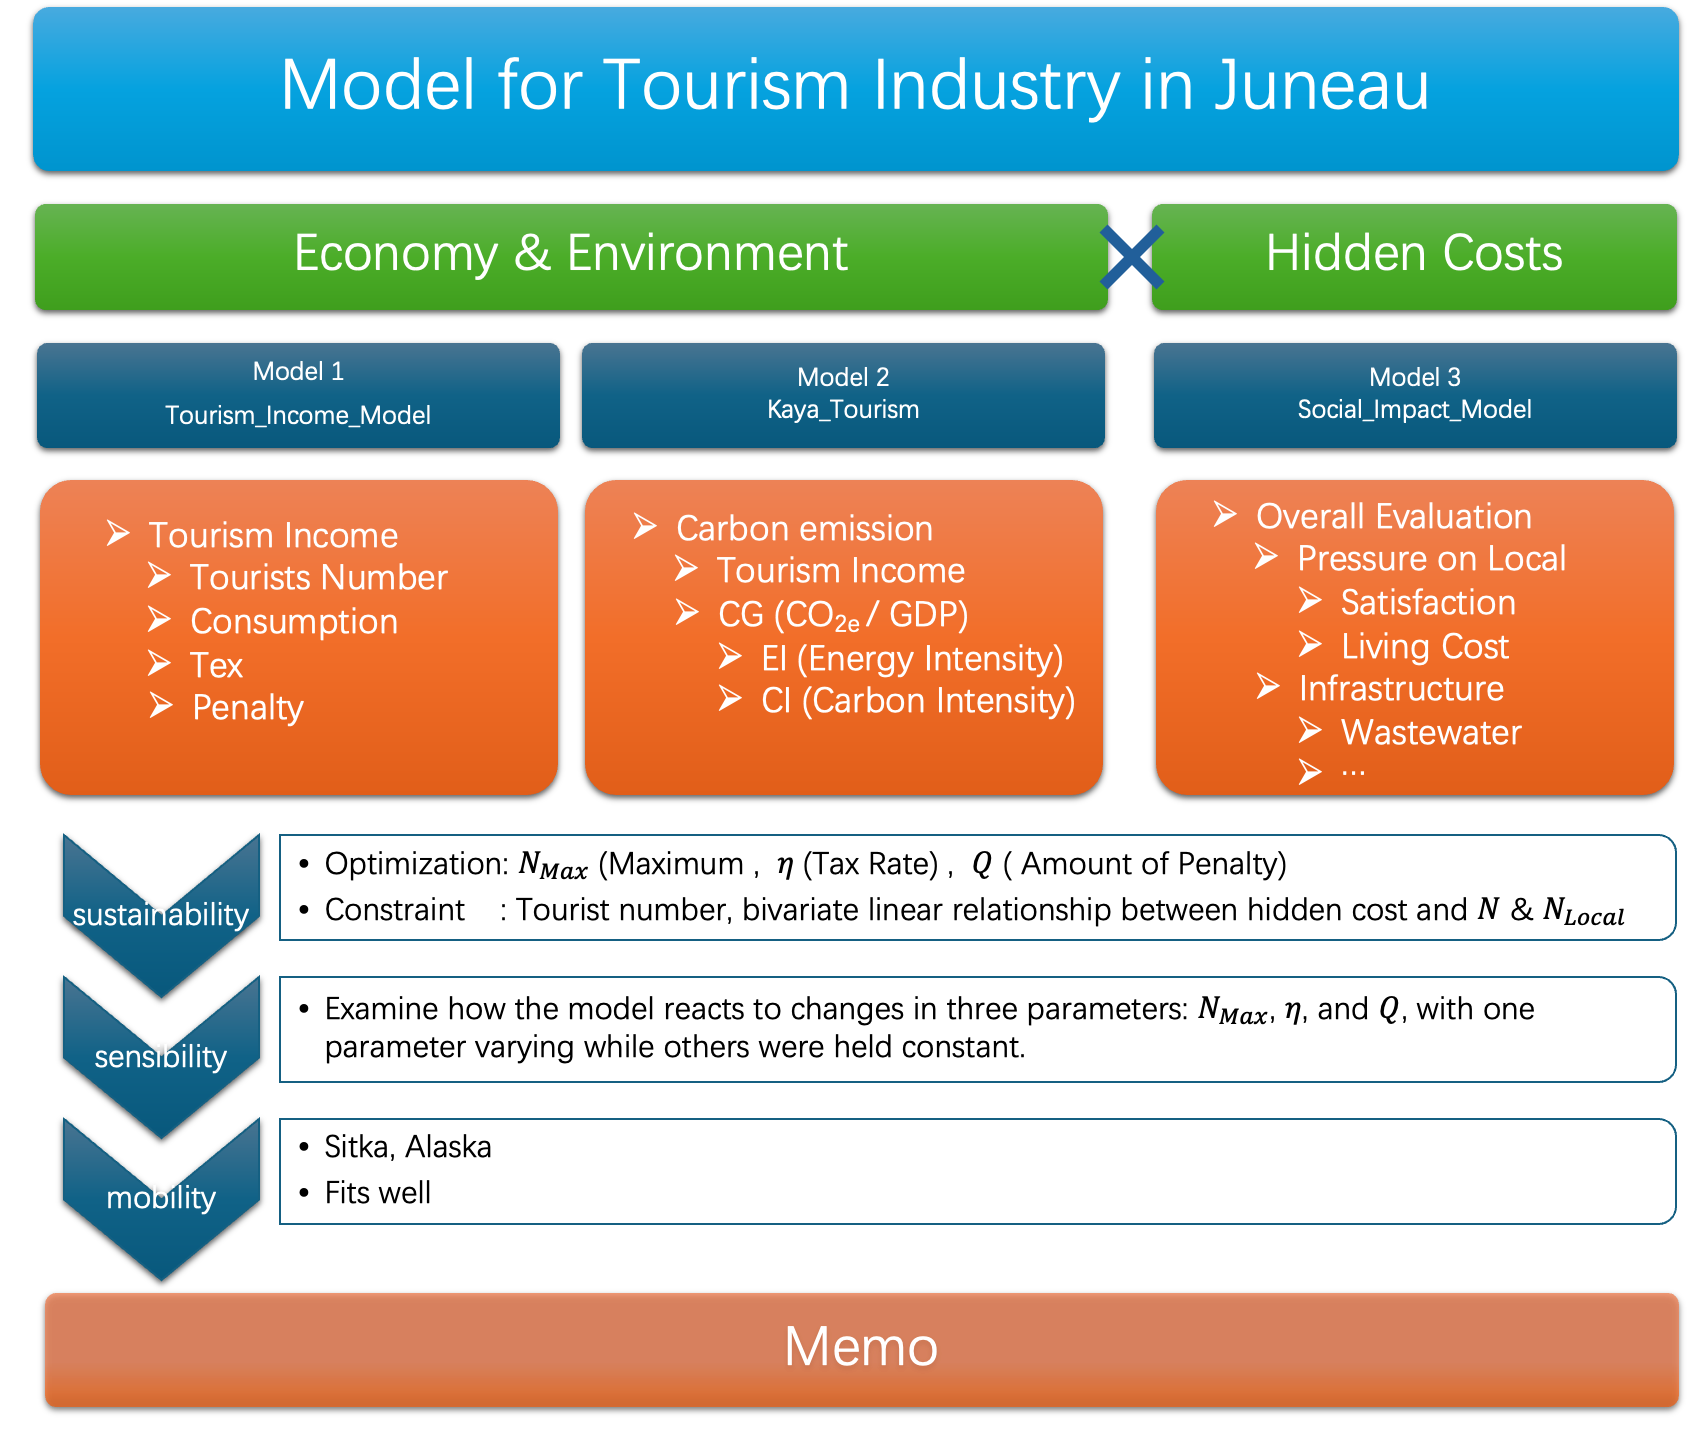
\includegraphics[width=1\textwidth]{FrameWork.jpg} % 插入图片
%     \caption{Our Work Overview Schematic Diagram}
% \end{figure}



\section{Assumptions and Notations}

\subsection{Assumptions}

The following reasonable assumptions are made to reasonably simplify the model:

\begin{itemize}
  \item Government policies (such as taxes, subsidies, regulations, etc.) remain unchanged during the period of the model.
  \item No major event compromising or promoting the tourism industry will occur during the period of our model.
  \item Consumer behavior, consumer preferences, or market demand are assumed to remain unchanged.
  \item Consumption per visitor per day remains stable.
\end{itemize}


\subsection{Notations}

The primary notations used in this paper are listed in Table 1.

\begin{table}[!htbp]
  \begin{center}
  \caption{Notations}
  \begin{tabular}{cc}
    \toprule
    \multicolumn{1}{m{3cm}}{\centering Symbol}
    &\multicolumn{1}{m{12cm}}{\centering Definition}\\
    \midrule
    $\eta$         &   tax rate\\
    $\mathcal{F}$         &   indicator of sustainability\\
    $Q$    &   amount of fine\\
    $\mathcal{I}$   &   social impact\\
    $N$    &   number of tourists (thousands)\\
    $N_{Local}$    &   number of local residents (thousands)\\
    $N_{Max}$    &   maximum number of tourists regulated (thousands)\\
    $CO_{2\_Tourism}$    &   carbon emissions from tourism\\
    $CG_{Tourism}$    &   tourism carbon emissions per GDP\\
    $CG_{All}$    &   carbon emissions per GDP\\
    \bottomrule
  \end{tabular}
  \end{center}
\end{table}

\section{Preliminary Analyses}


We first analyse the potential factors that may affect the tourism industry in Juneau, thus enabling
 a smoother transition to the model building process.

 \subsection{Number of Tourists}

 We found no existing data on the number of tourists visiting Juneau each year, but we can infer it
 by other means.

 According to [1] and [2], among all the transportation methods, cruise ships are the most popular way to visit Juneau,
 accounting for over 90\% of the total number of tourists. As the number of cruise ship passengers is available online, 
 we can use it as a proxy to estimate the total number of tourists.

According to [3], the number of cruise ship passengers visiting Juneau is as follows:

 \begin{table}[H]
    \centering
    \renewcommand{\arraystretch}{1.3}
    \caption{Number of Cruise Ship Visitors to Juneau}
 \begin{tabular}{|c|c|c|c|c|c|c|c|c|c|c|}
    \hline \textit{Year} & 2014 & 2015 & 2016 & 2017 & 2018 & 2019 & 2020 & 2021 & 2022 & 2023 \\
    \hline \begin{tabular}{l} 
    \textit{Num(in thousands)} 
    \end{tabular} & 961 & 983 & 1015 & 1072 & 1151 & 1306 & 0 & 117 & 1167 & 1670 \\
    \hline
    \end{tabular}
\end{table}
It can be easily noted that numbers plummeted in 2020 and 2021 due to the COVID-19 pandemic.
In this section, we use the \textit{SARIMAX} model including the pandemiuc factor to 
predict the number of tourists in the next few years.

\subsubsection{SARIMAX Model}

The \textit{SARIMAX} model, which stands for \textit{Seasonal AutoRegressive Integrated 
Moving Average with eXogenous regressors}, is an extension of the \textit{ARIMA}
 \textit{(AutoRegressive Integrated Moving Average)} model that incorporates seasonal 
 effects and external variables. Since we need to consider the impact factors during the 
 pandemic, \textit{SARIMAX} is used instead of \textit{ARIMA}.

\subsubsection{Parameters Setting}

\begin{itemize}
    \item \textbf{Pandemic Impact Factor}: Given the severity of the COVID-19 pandemic, different factors are set.
    In 2020, 2021 when the pandemic was at its peak, factors are set to 1, in 2021 set to 0.3, and in other years set to 0.
    \item \textbf{Order (p, d, q)}: The order of the ARIMA part of the model is set to (2, 1, 1) after conducting the ACF and PACF analysis(see Figure 1).
    \item \textbf{Enforce Stationarity}: The enforce$\_$stationarity parameter is set to True to ensure the model is stationary.
    \item \textbf{Enforce Invertibility}: The enforce$\_$invertibility parameter is set to True to ensure the model is invertible.
\end{itemize}

\subsubsection{Model Results}

The \textit{SARIMAX} model is trained on the data from 2014 to 2023 
and used to predict the number of tourists in the next few years.
The prediction result is lited as follows. The residuals, ACF and PACF plots are 
also shown in Figure 1.

\begin{figure}[H]
    \centering
    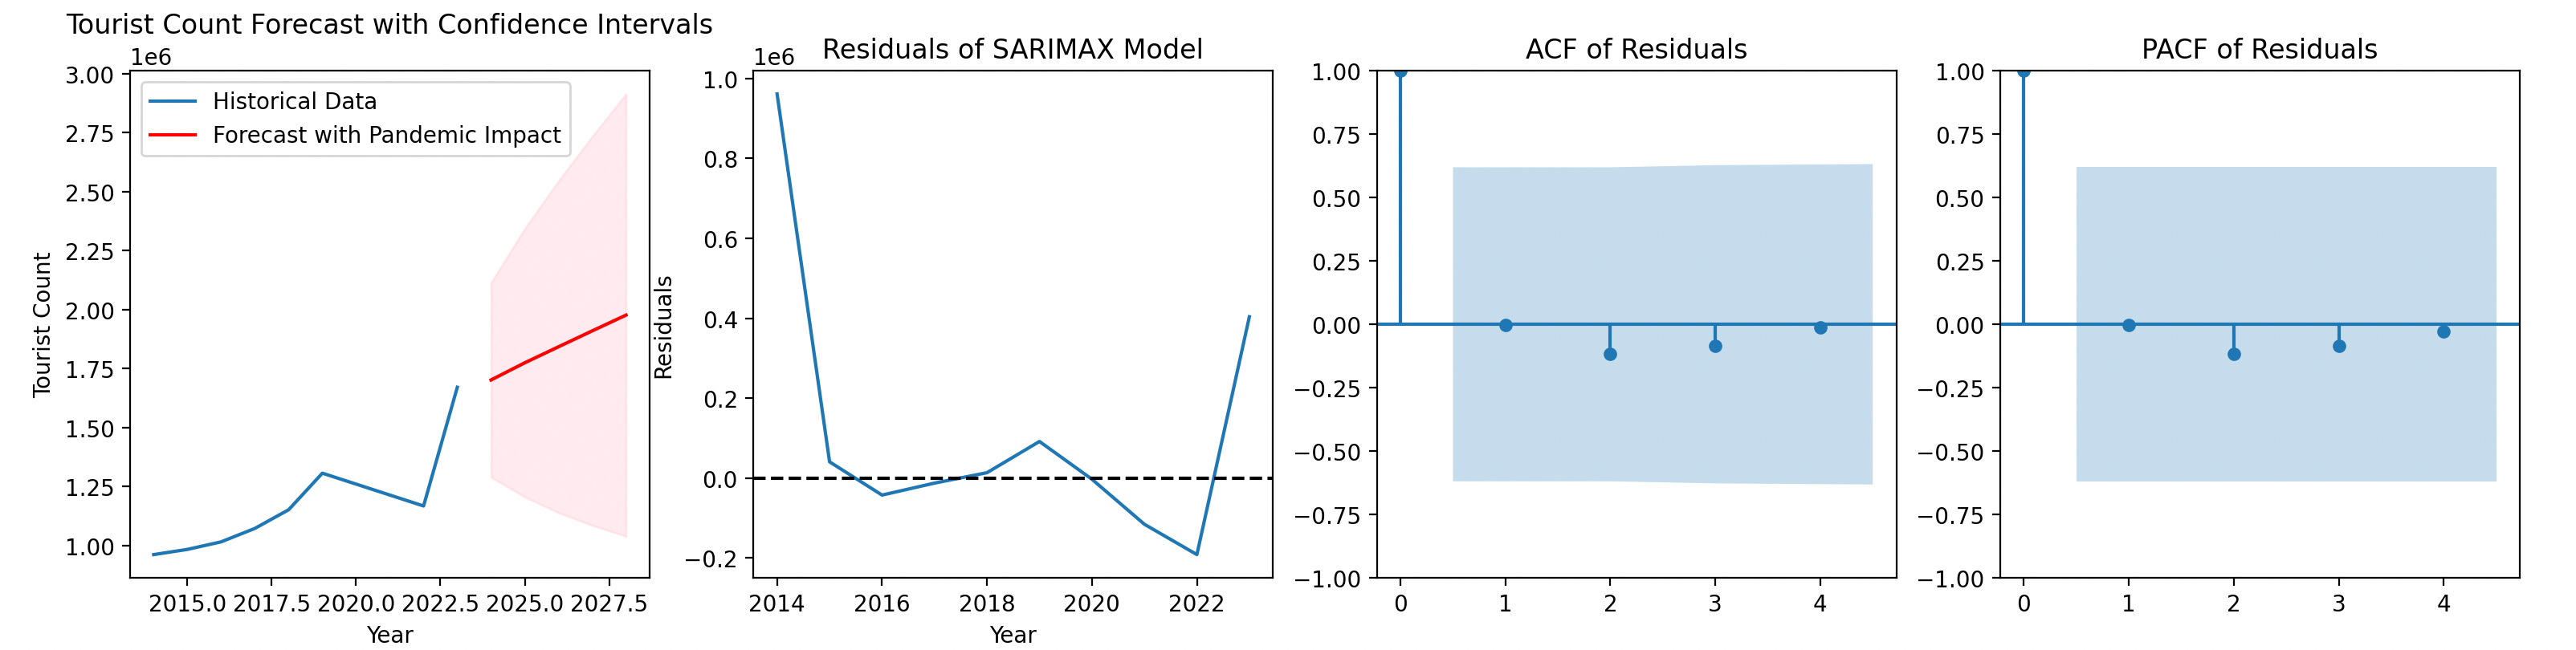
\includegraphics[width=1\textwidth]{Fig_Tourists.jpg} % 插入图片
    \vspace{-0.4cm}
    \caption{Tourist Prediction}
\end{figure}

It can be seen that the model correctly handles the plummet during the pandemic and
captures the trend of the revival of tourism. The exact number of 
tourists in the next few years is shown below, which will be utilized in the following sections.

\begin{table}[H]
    \centering
    \caption{Number of Tourists Prediction}
    \renewcommand{\arraystretch}{1.3}
 \begin{tabular}{|c|c|c|c|c|c|}
    \hline \textit{Year} & 2024 & 2025 & 2026 & 2027 & 2028 \\
    \hline \begin{tabular}{l} 
    \textit{Num(in thousands)} 
    \end{tabular} & 1701 & 1774 & 1842 & 1909 & 1976 \\
    \hline
    \end{tabular}
\end{table}



\subsection{Number of Local Residents}

\subsubsection{Population of Juneau}

According to \textit{World Population Review}, the population of Juneau in the last decade is as follows:

\begin{table}[H]
    \centering
    \caption{Population of Juneau}
    \renewcommand{\arraystretch}{1.3}
    \resizebox{\textwidth}{!}{
    \begin{tabular}{|c|c|c|c|c|c|c|c|c|c|c|c|c|c|c|c|}
        \hline \textit{Year} & 2010 & 2011 & 2012 & 2013 & 2014 & 2015 & 2016 & 2017 & 2018 & 2019 & 2020 & 2021 & 2022 & 2023 & 2024 \\
        \hline \textit{Num (in thousands)} & 31.4 & 32.2 & 32.4 & 32.6 & 32.5 & 32.6 & 32.5 & 32.1 & 32.0 & 32.0 & 32.2 & 32.0 & 31.7 & 31.6 & 31.3 \\
        \hline
    \end{tabular}
    }
\end{table}

\subsubsection{Population Prediction}

We still use the \textit{SARIMAX} model proposed in the last section
to predict the population of Juneau in the next few years. Parameters are the same as the last section.
The first four pictures are still the original data and predicted data, the residual, ACF and PACF plots.
In addition, official prediction data can also be found in \textit{World Population Review}, therefore two additional pictures are added to compare the prediction results.

\begin{figure}[H]
    \centering
    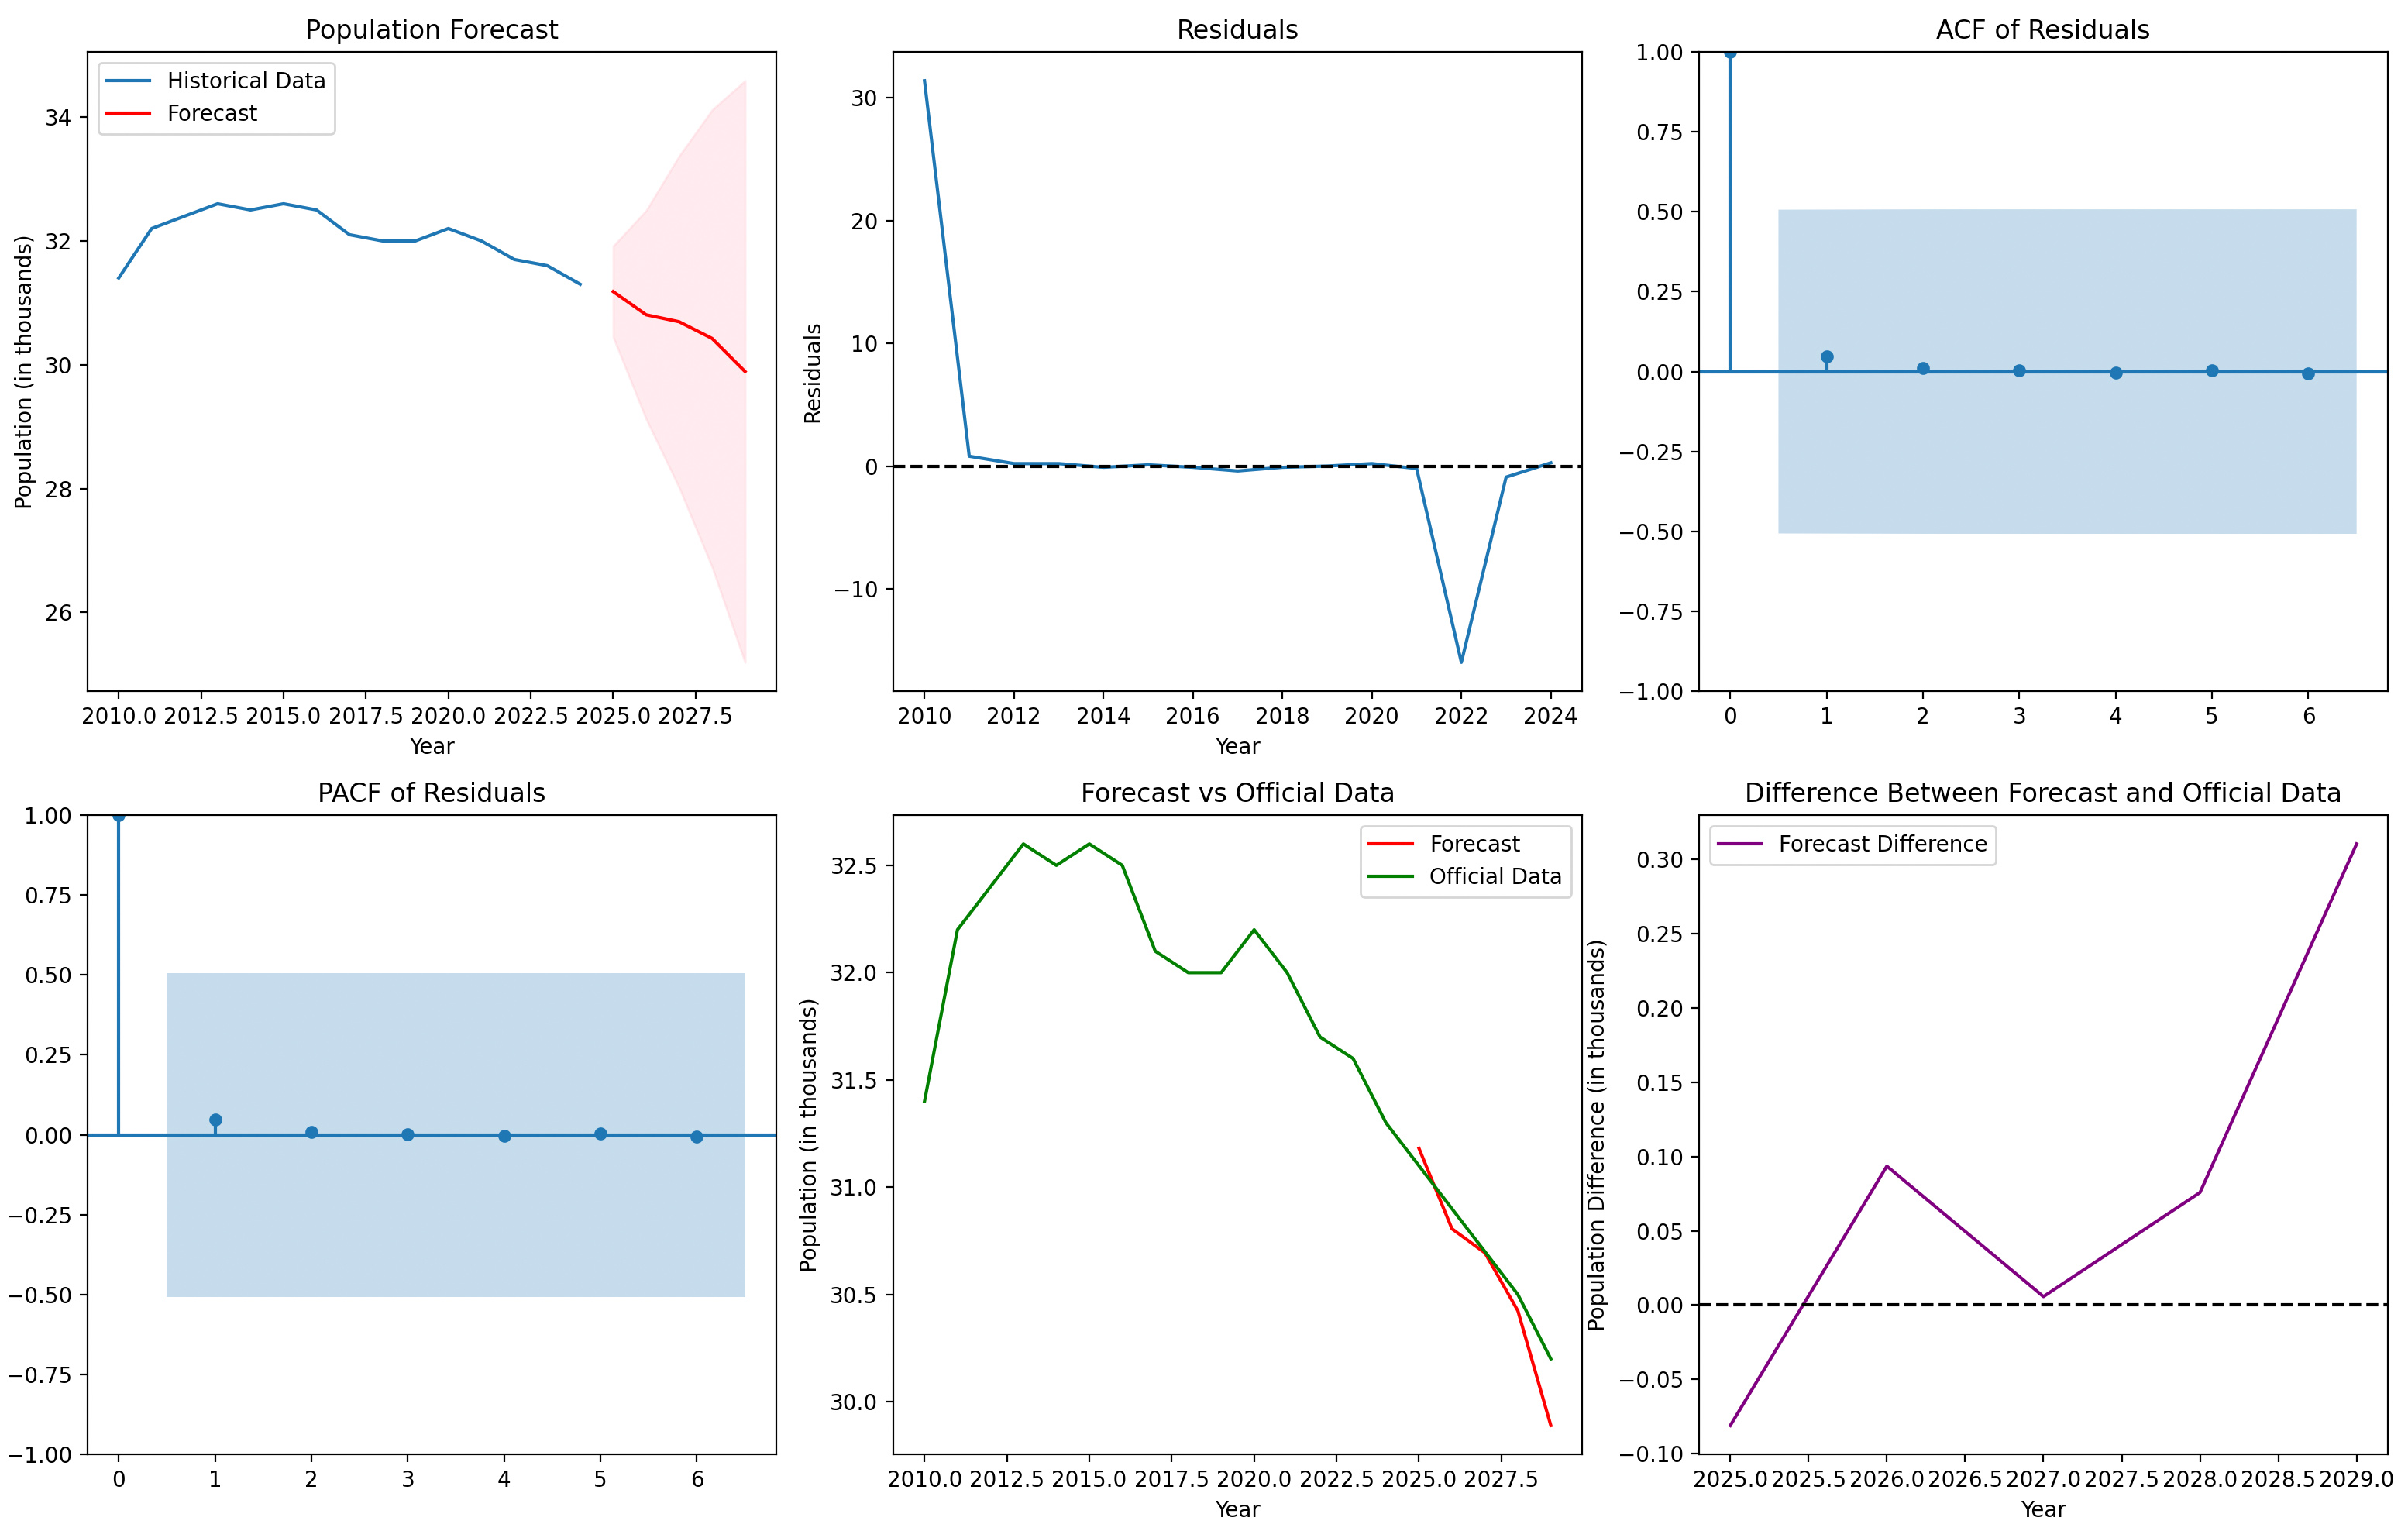
\includegraphics[width=1\textwidth]{Fig_Population.jpg} % 插入图片
    \vspace{-0.4cm}
    \caption{Tourist Prediction}
\end{figure}

It can be concluded from subfigure 5 and 6 that the model fits the data well 
and the prediction is reliable. The exact number of local residents in the next 
few years is shown below.

\begin{table}[H]
    \centering
    \caption{Population Prediction}
    \renewcommand{\arraystretch}{1.3}
 \begin{tabular}{|c|c|c|c|c|c|}
    \hline \textit{Year}  & 2025 & 2026 & 2027 & 2028 & 2029\\
    \hline \begin{tabular}{l} 
    \textit{Num(in thousands)} 
    \end{tabular} & 31.2 & 30.8 & 30.7 & 30.4 & 30.0 \\
    \hline
    \end{tabular}
\end{table}


\clearpage


\section{问题一:两组专家对同批教师教学评价的差异性与可信度分析}


\subsection{建模思路与分析流程}
本节思路如下:

\begin{enumerate}
    \item \textbf{数据预处理与批量求和}:针对原始多层次评分表,对每位教师、每组专家的11项具体指标分数求和,得出教师—专家—组的总分数据。对于极个别缺失情况,采用“同一教师该指标其他专家均值补齐”策略,确保数据完整性。
    \item \textbf{描述性统计分析}:对两组专家评分总分计算均值、中位数、标准差、极差、偏度、峰度等,并通过箱线图、直方图展示分布,为后续检验提供支持。
    \item \textbf{显著性差异检验与效应量分析}:考虑到数据为同一批教师的配对评分,首先进行差值的正态性检验(Shapiro-Wilk),如通过则用配对t检验,否则用Wilcoxon符号秩检验。进而计算Cohen's $d$,定量衡量实际意义。
    \item \textbf{内部一致性与可信度评价}:采用组内相关系数ICC(双向随机效应、绝对一致性、单次测量模型 ICC(2,1)),分析每组专家评分的一致性,值越大可信度越高。
    \item \textbf{综合判据与结论}:整合差异显著性、效应大小与ICC,系统比较两组专家数据的可靠性。
\end{enumerate}

\subsection{数据处理与描述性统计}


\begin{itemize}
    \item $n$:参评教师人数。
    \item $S^{(1)}_i$:第$i$位教师第一组专家的平均总分。
    \item $S^{(2)}_i$:第$i$位教师第二组专家的平均总分。
    \item $D_i = S^{(1)}_i - S^{(2)}_i$:第$i$位教师两组评分平均值差异。
\end{itemize}

\begin{figure}[htbp]
    \centering
    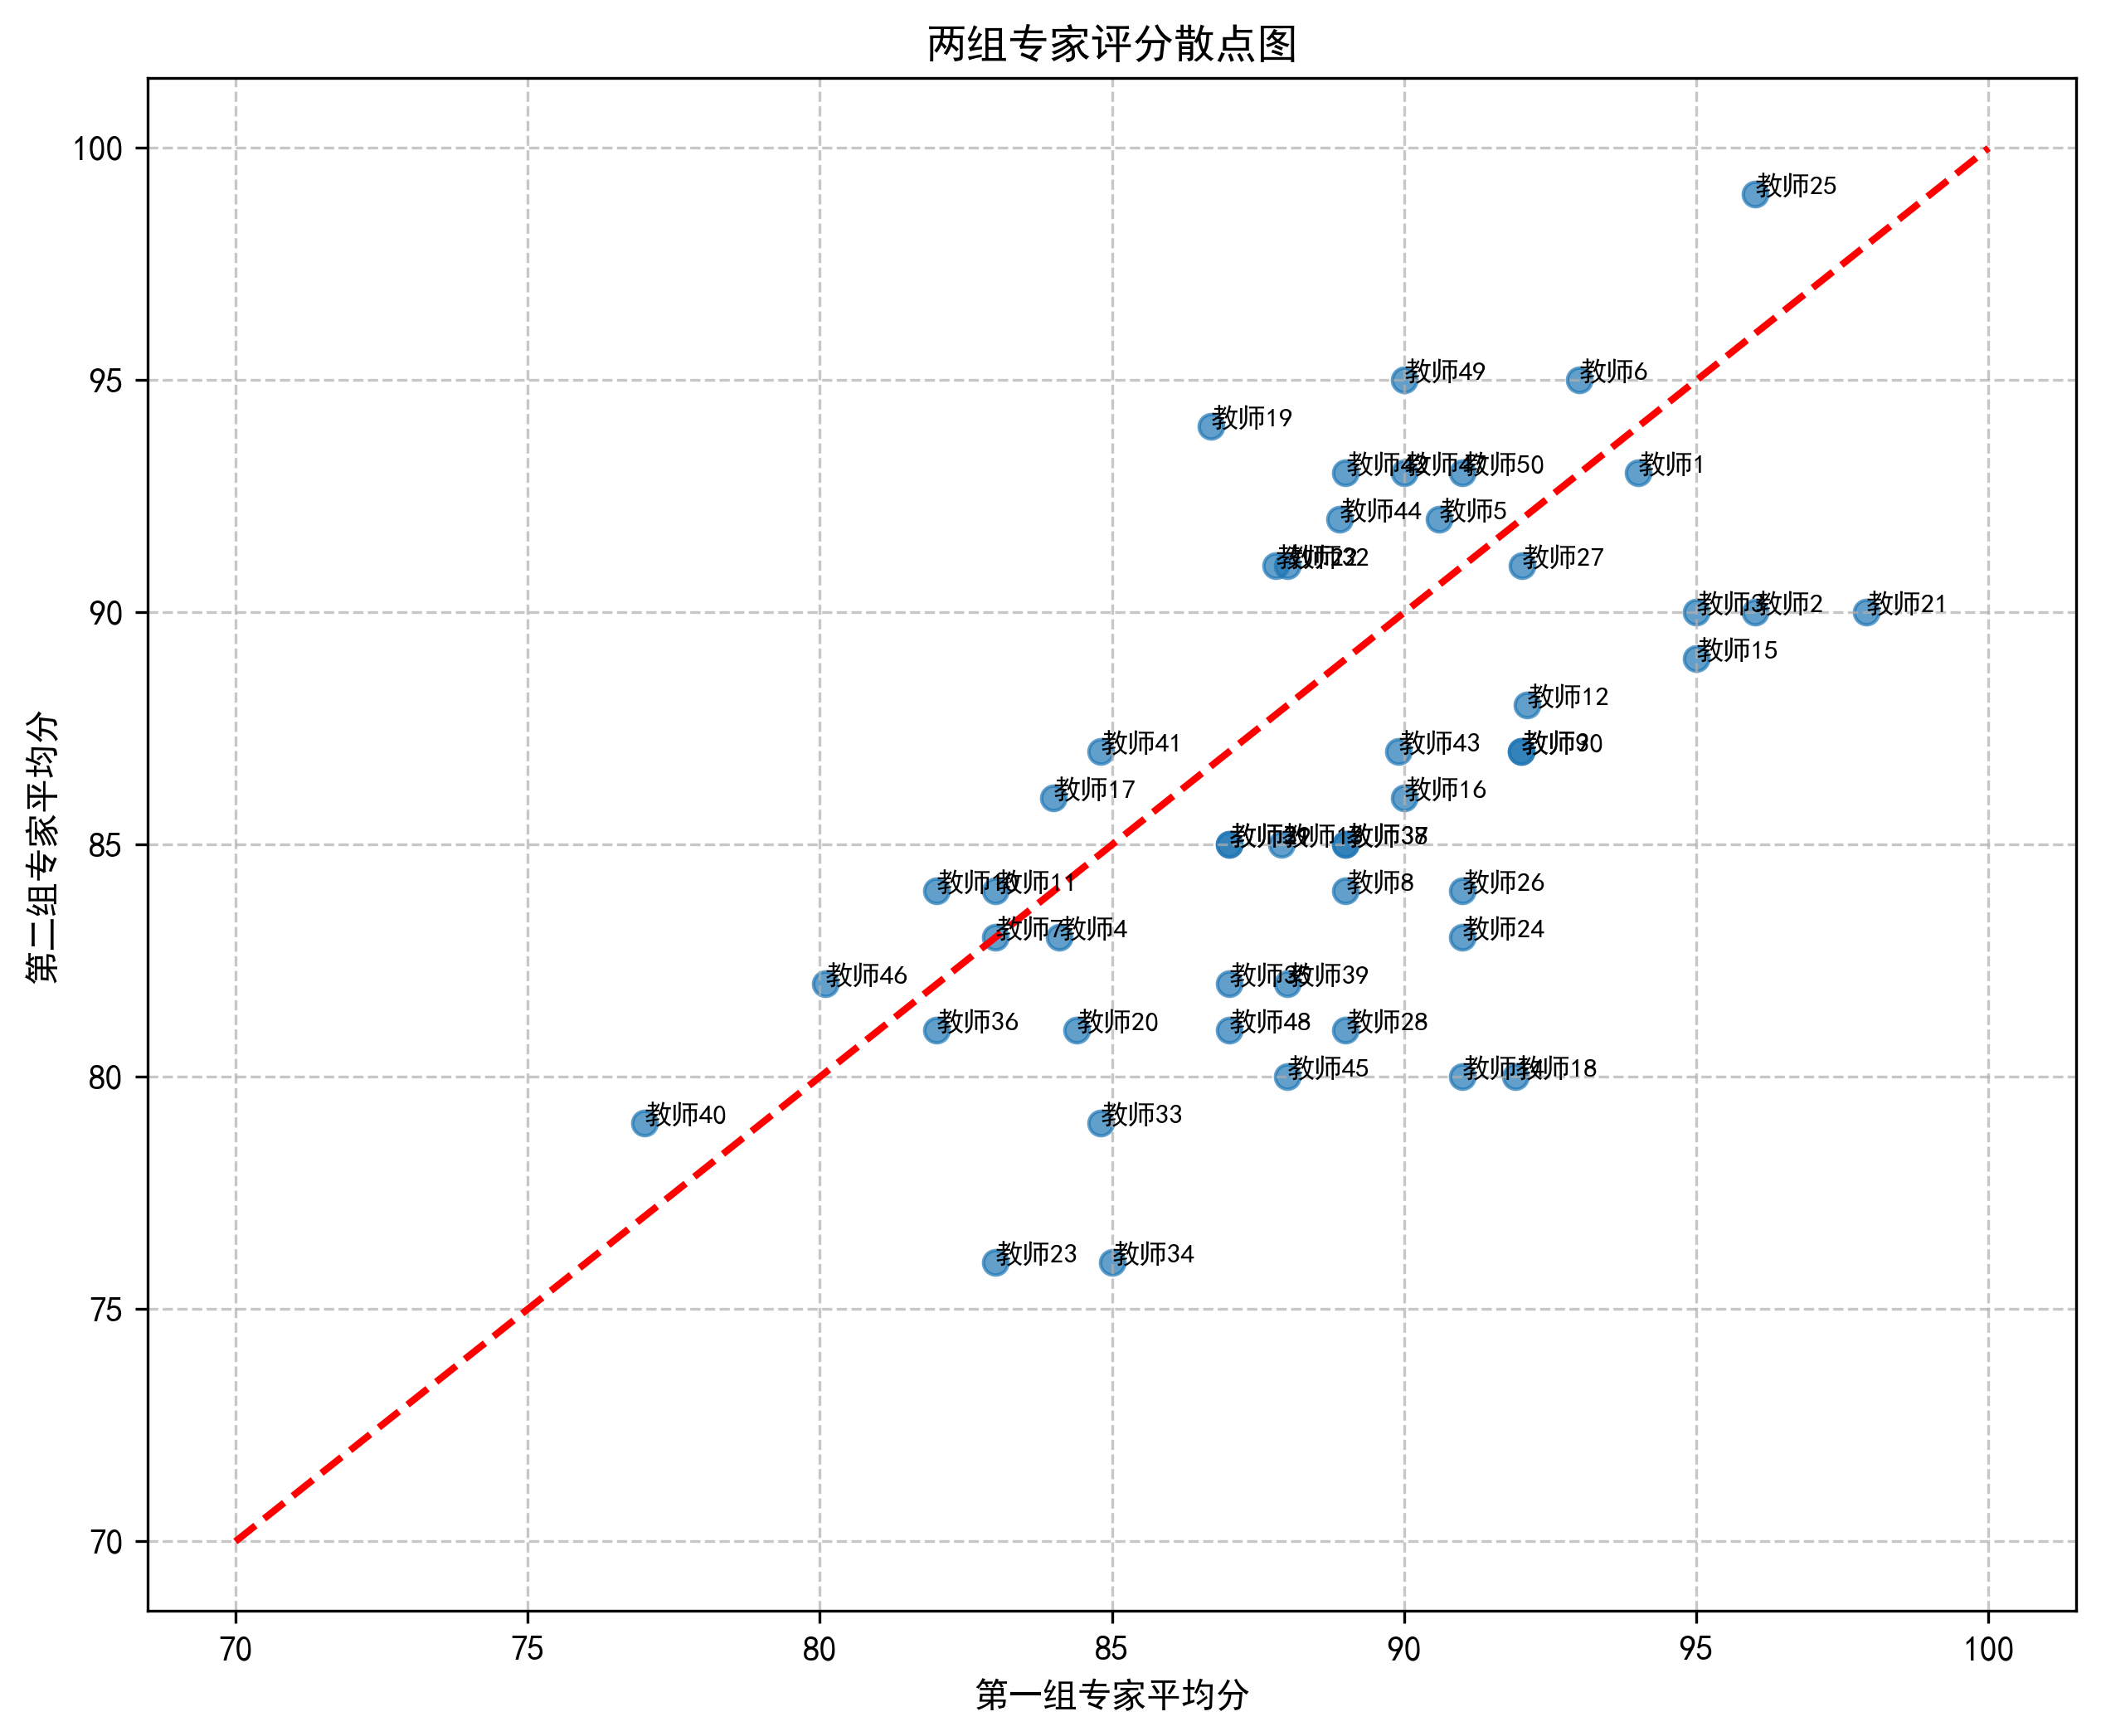
\includegraphics[width=0.6\textwidth]{scores_scatter.png} % 插入图片
    \caption{散点图}
\end{figure}


统计并对比两组评分的均值、标准差、极差、偏度、峰度等核心指标,并辅以箱线图、直方图等可视化手段直观展示分布形态、中心趋势、离散程度和潜在异常,为后续推断检验和一致性评估奠定基础。

\begin{figure}[htbp]
    \centering
    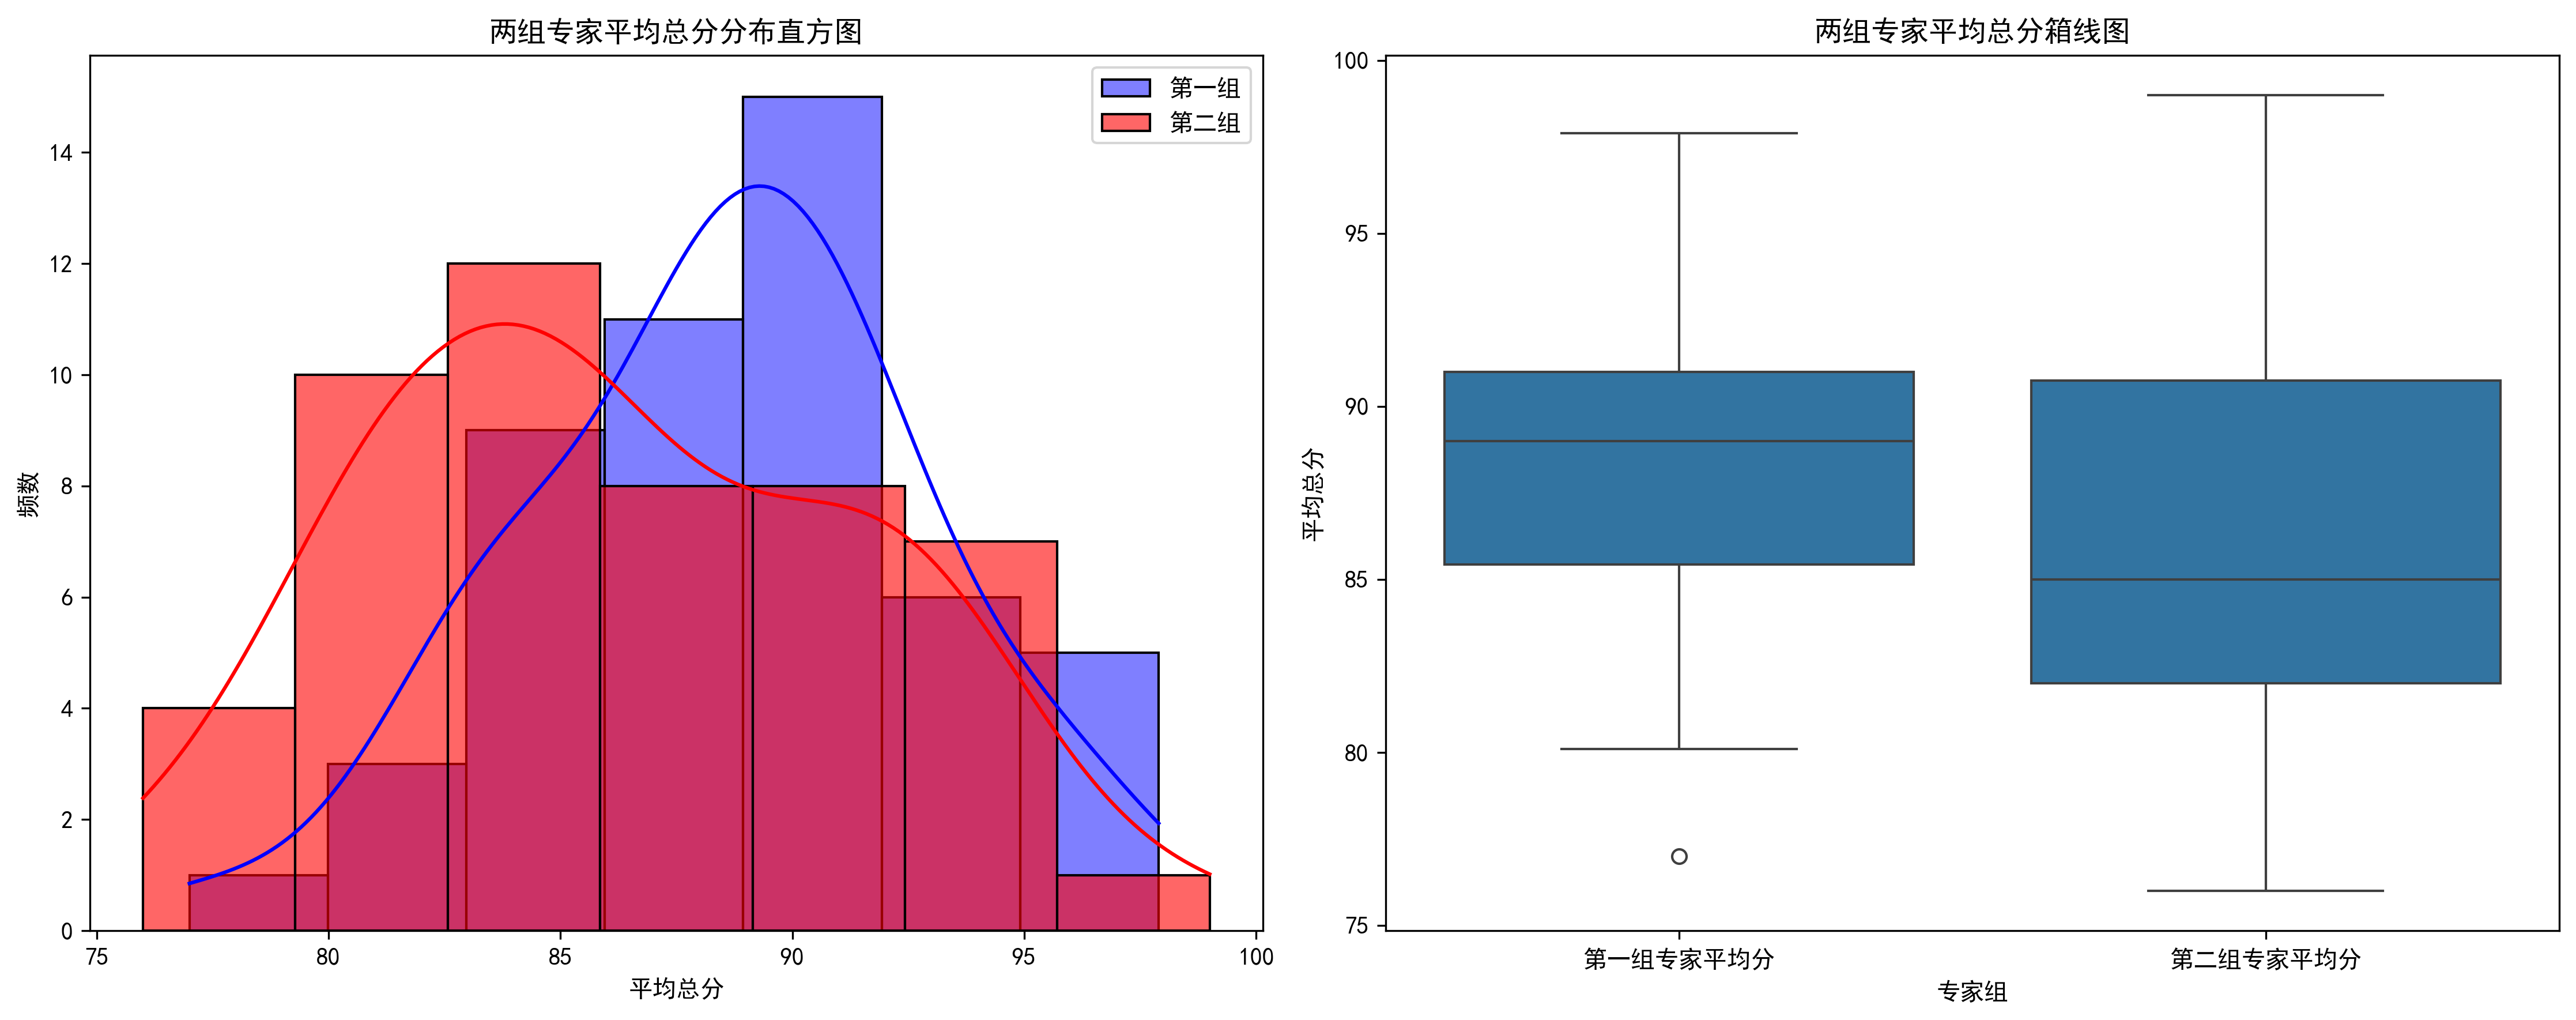
\includegraphics[width=1\textwidth]{descriptive_statistics.png} % 插入图片
    \caption{直方图和箱线图}
\end{figure}



对所有教师-专家数据,经清洗和缺失项均值填补后,分别求得两组专家每位教师的平均总分 $S^{(1)}_i, S^{(2)}_i$。以附件1为例,第一组专家评分均值88.54,标准差4.34,第二组均值86.18,标准差5.35,均略呈负偏态。表~\ref{tab:descstat} 总结描述性统计结果。



\begin{table}[h]
\centering
\caption{两组专家评分描述性统计}
\label{tab:descstat}
\begin{tabular}{lcc}
\toprule
统计指标 & 第一组专家评分 & 第二组专家评分 \\
\midrule
样本量      & 50        & 50        \\
均值        & 88.54     & 86.18     \\
标准差      & 4.34      & 5.35      \\
最小值      & 77.00     & 76.00     \\
极差        & 20.90     & 23.00     \\
偏度        & -0.23     & 0.23      \\
峰度        & -0.05     & -0.68     \\
\bottomrule
\end{tabular}
\end{table}

\subsection{显著性差异检验与效应量}
\subsubsection{配对显著性检验}
针对同一批教师的配对评分,先对两组评分差值$D_i$进行Shapiro-Wilk正态性检验。若近似正态,采用配对$t$检验对两组均值差异做统计推断;若非正态,则采用Wilcoxon符号秩检验。以$p$值小于0.05为统计显著,结合效应量判断实际意义。

\subsubsection{效应量量化}
采用配对样本下的Cohen's $d$量化两组专家均值差异的实际影响:
\[
d = \frac{\overline{D}}{s_D}
\]
其中$\overline{D}$为所有差值均值,$s_D$为样本标准差。$|d| \approx 0.2$为小效应,$\approx 0.5$为中等效应,$\approx 0.8$为大效应,这可弥补$p$值无法揭示实际影响大小的不足。

教师的两组专家平均分之差 $D_i = S^{(1)}_i - S^{(2)}_i$ 经Shapiro-Wilk检验$p=0.187$,近似正态,适合配对样本t检验。t检验$p=0.001$,两组专家评分存在统计学显著差异。Cohen's $d=0.52$,为中等效应,说明分组差异在实际教学评价中具备一定意义。

\subsection{专家组可靠性(内部一致性)分析}
采用组内相关系数ICC(Intraclass Correlation Coefficient)定量评价组内一致性。模型选用“双向随机效应、绝对一致性、单次测量”ICC(2,1)标准,是因为:

\begin{itemize}
    \item 双向随机效应假设专家和被评分教师均为总体的随机抽取,增强结论的普适性;
    \item 绝对一致性着重考察分数本身(非仅排名)的一致水平;
    \item 单次测量聚焦个别评分者一致性(适合专家组实际结构)。
\end{itemize}

ICC判据:$<0.5$为差;$0.5{\sim}0.75$为中等;$0.75{\sim}0.9$良好;$\geq0.9$优秀。

\begin{figure}[H]
    \centering
    \begin{minipage}[t]{0.5\textwidth}
        \centering
        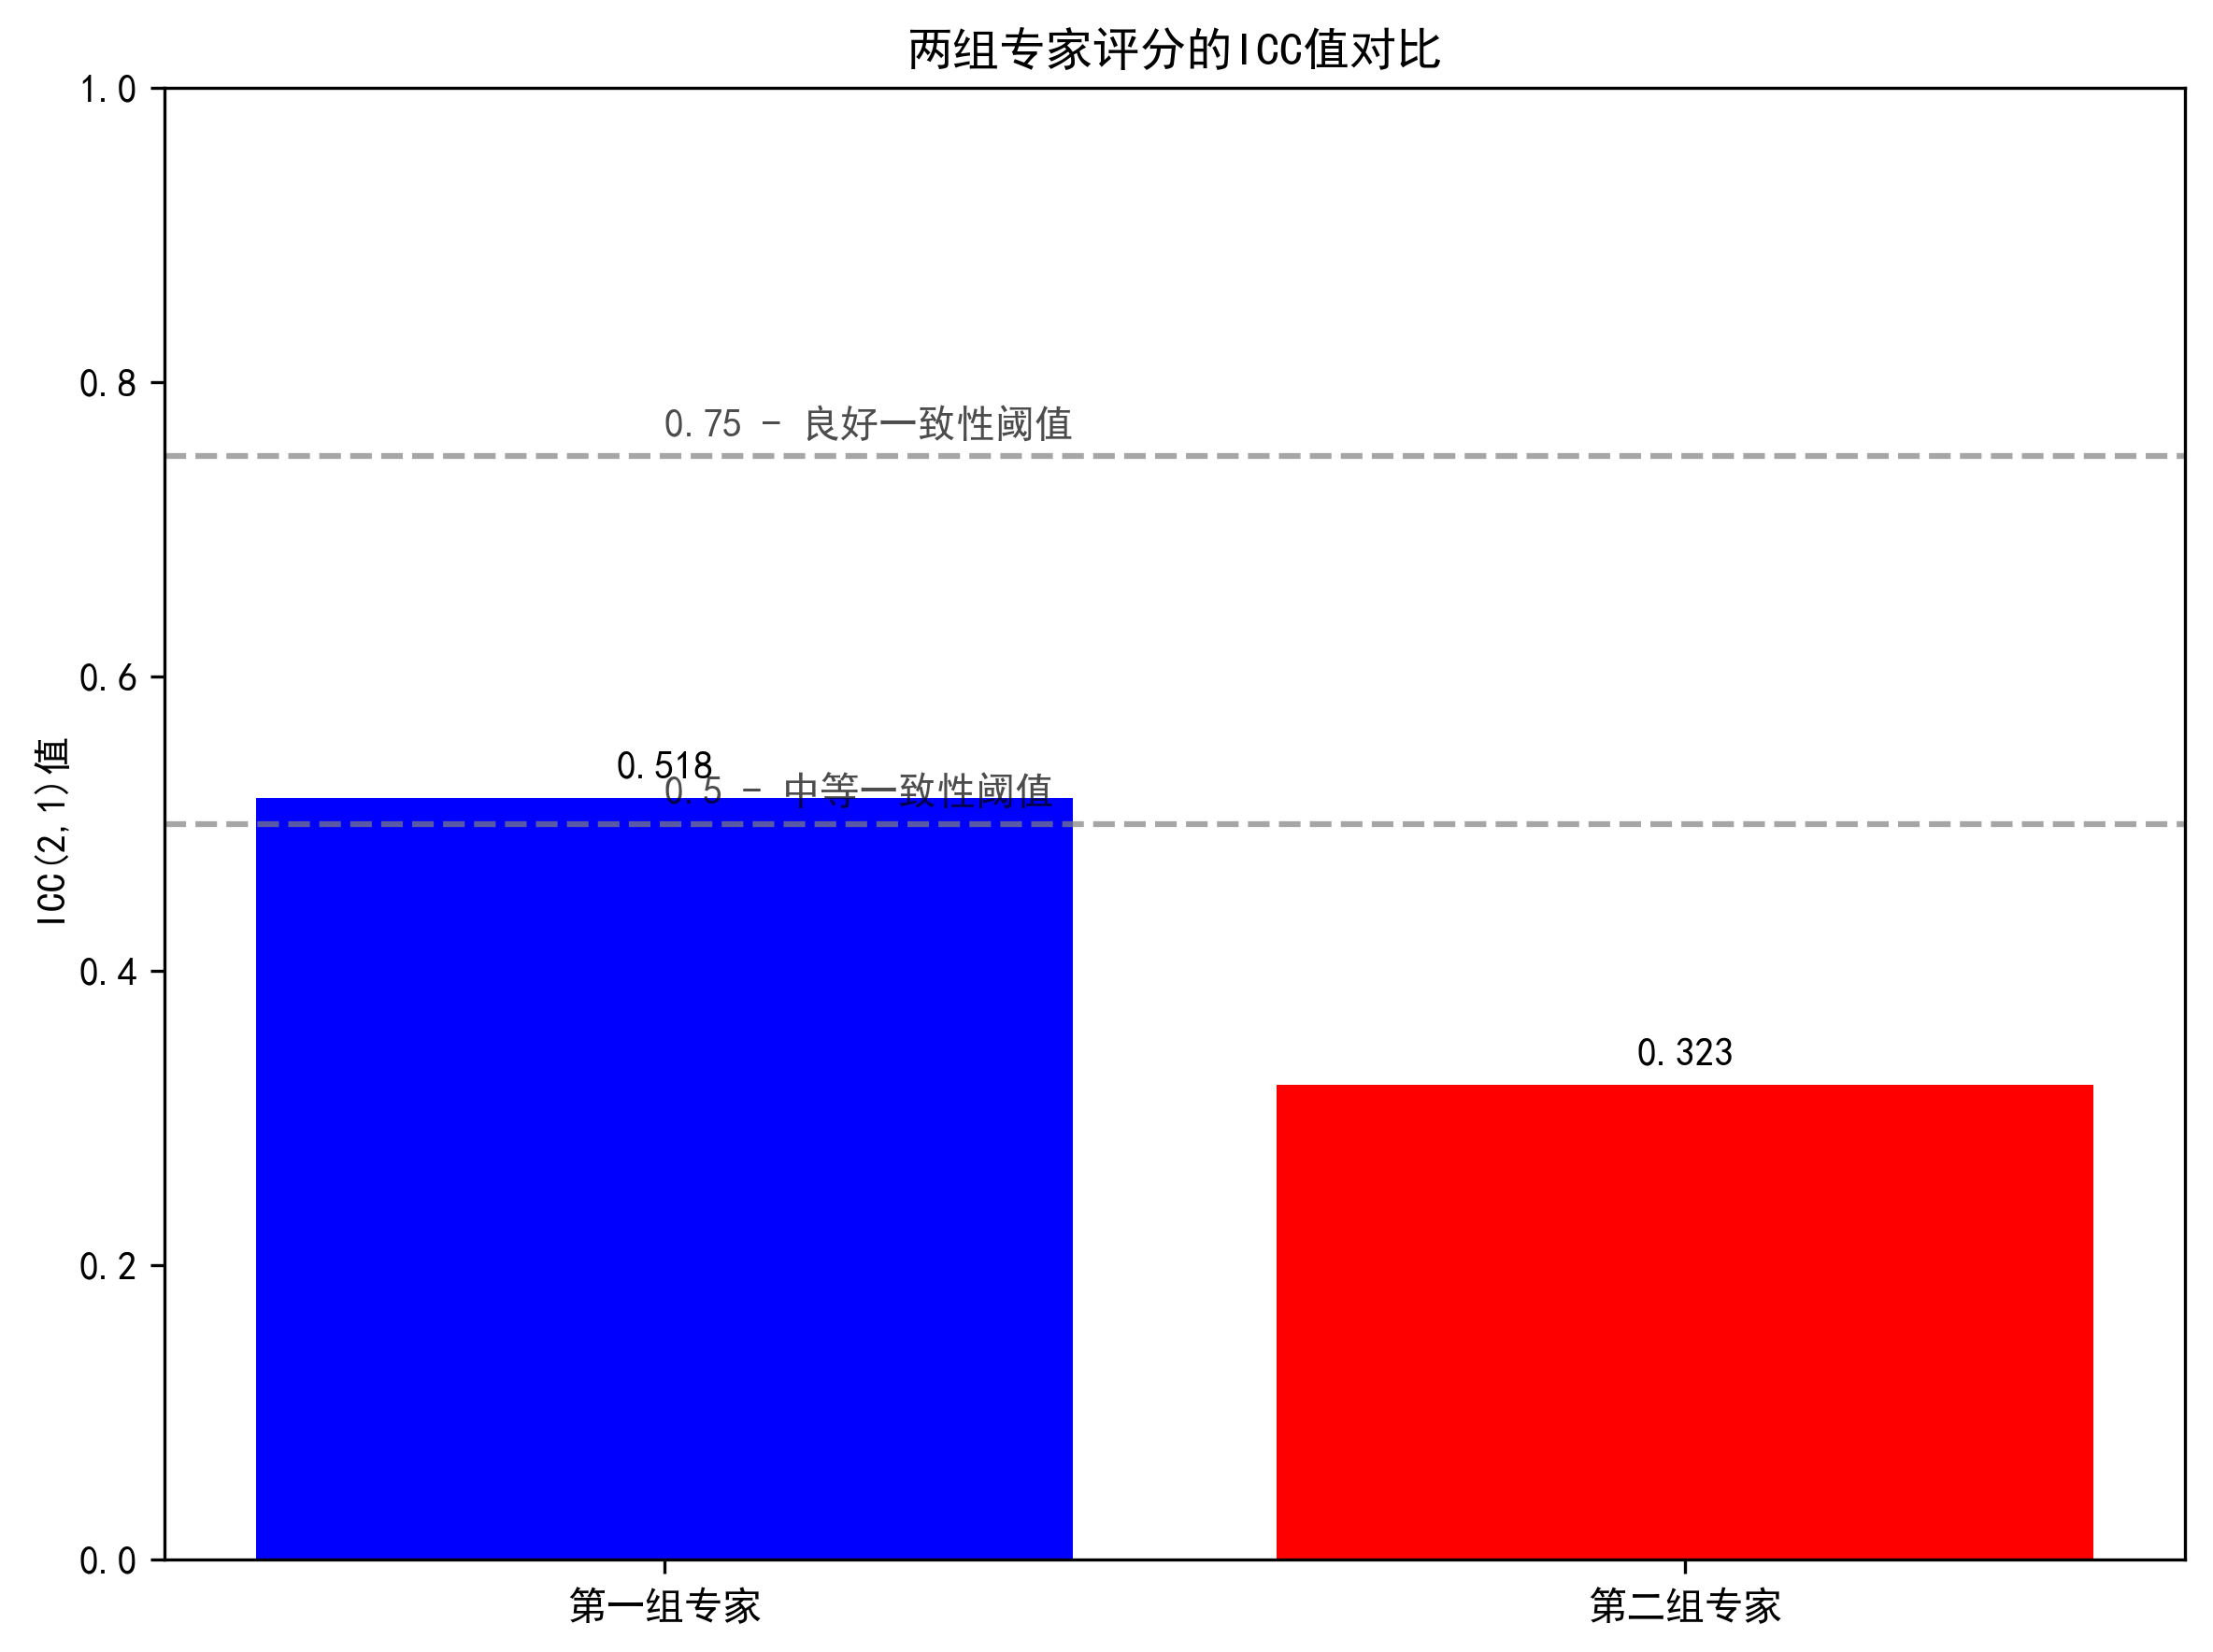
\includegraphics[width=1\textwidth]{icc_analysis.png}
    \end{minipage}
    \hfill
    \begin{minipage}[t]{1\textwidth}
        \centering
        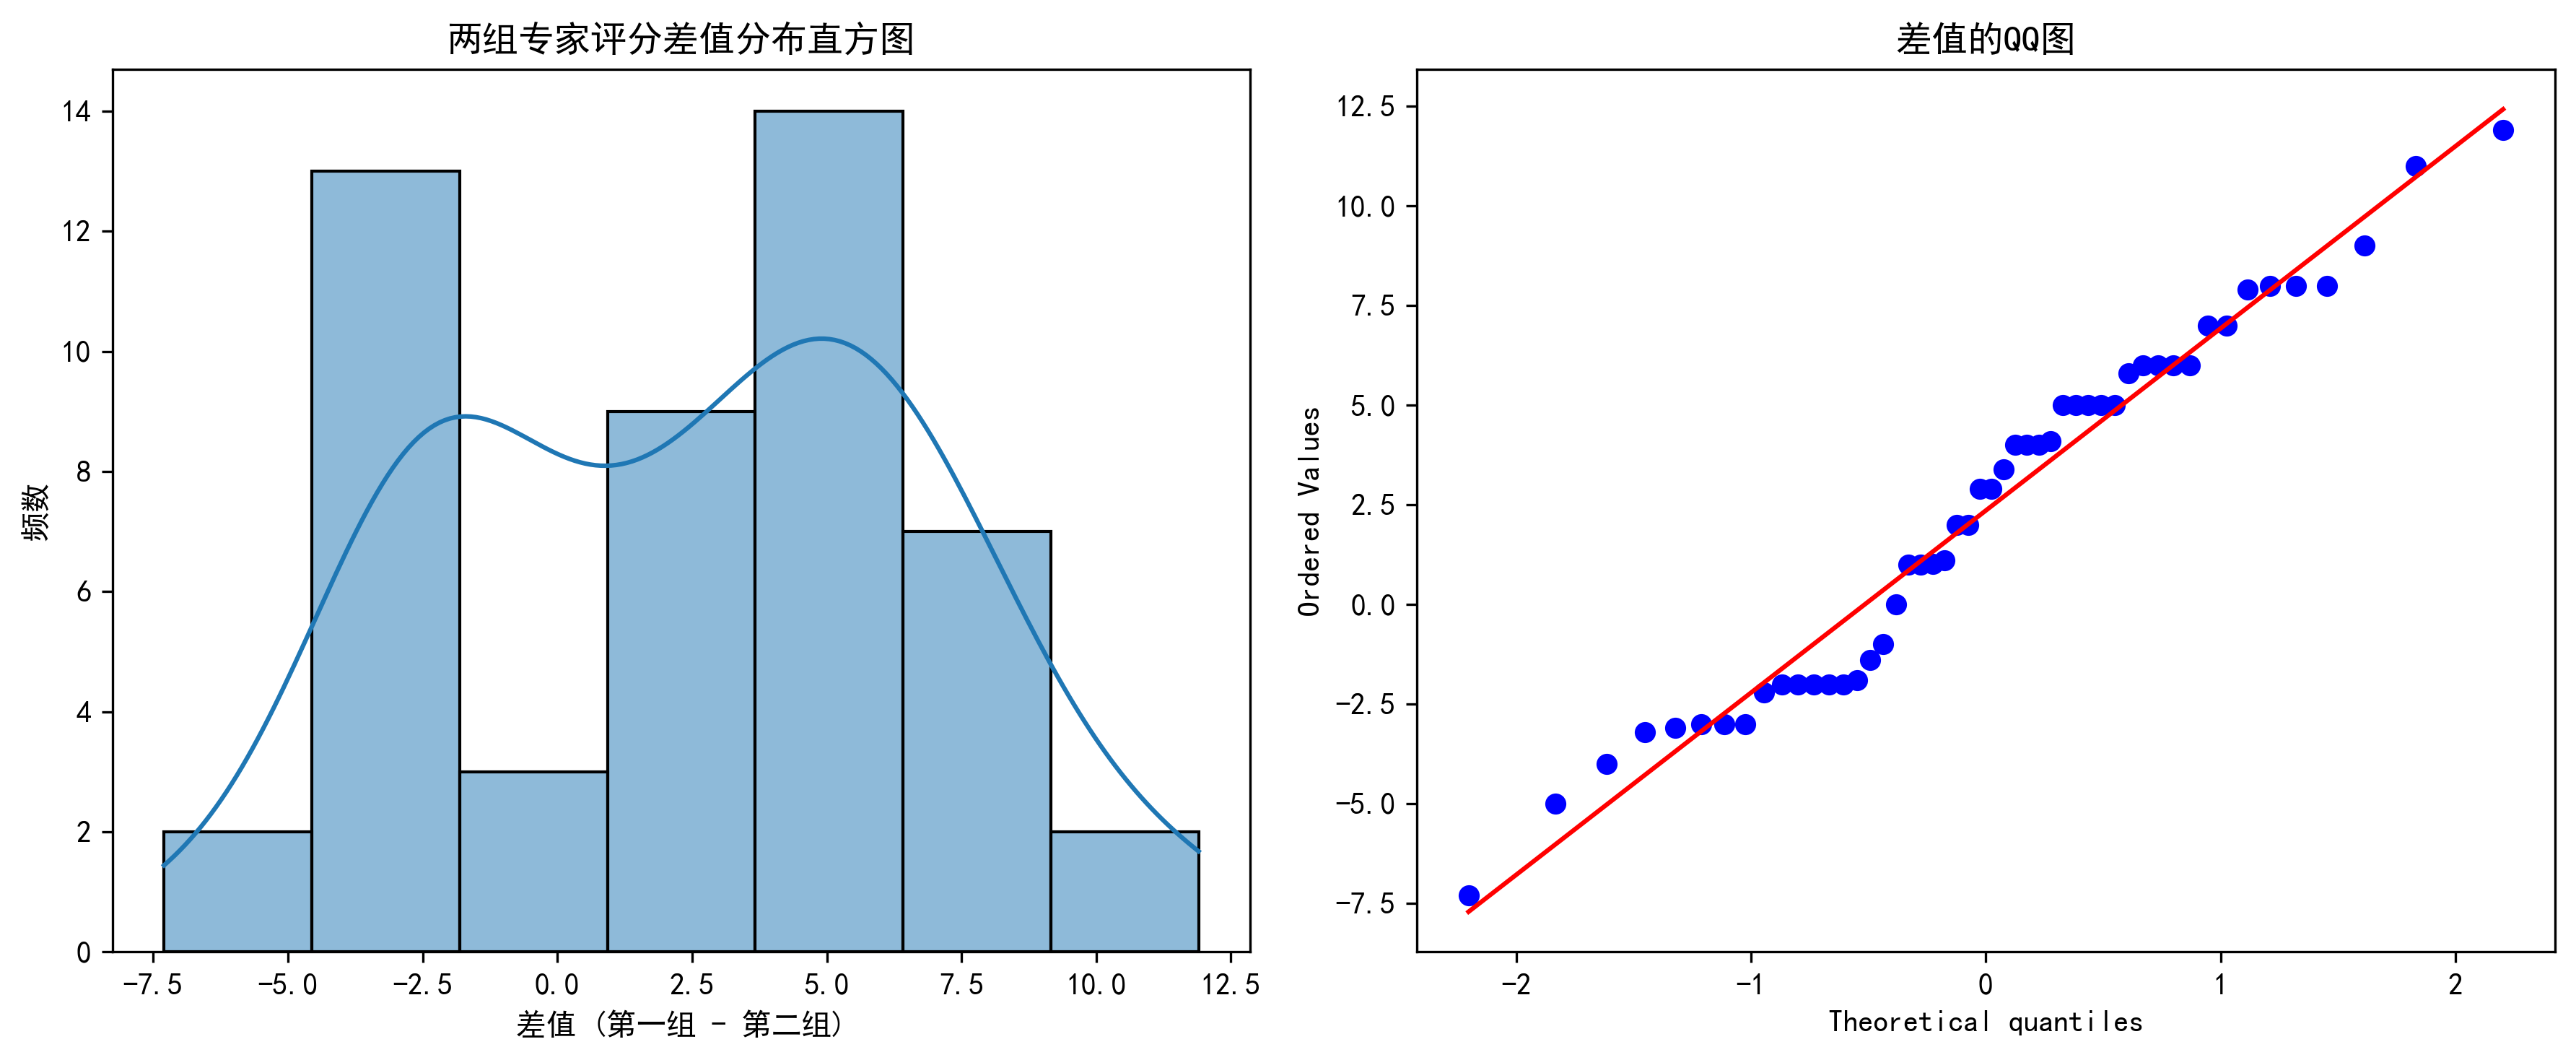
\includegraphics[width=1\textwidth]{normality_test.png}
    \end{minipage}
\end{figure}


分别计算两组专家内ICC(双向随机效应、绝对一致性、单次测量):
\begin{itemize}
    \item 第一组ICC=0.518(中等一致性)
    \item 第二组ICC=0.323(差/不可接受的一致性)
\end{itemize}
第一组专家在评分标准和评分稳定性方面表现更优,具有更高的一致性和集体信度。

\subsection{综合判断与结论}
以实际分析为例,经描述性统计,第一组均值高于第二组(88.54 vs 86.18),标准差更低。差值$D_i$正态性检验$p=0.187$,支持采用配对$t$检验,检验$p=0.001$,存在显著差异。Cohen's $d=0.522$,为中等效应。

ICC分析显示,第一组ICC=0.518(中等一致性),第二组ICC=0.323(偏低一致性)。表明第一组专家判分标准更统一、一致性更优,具备更高集体信度。

本节通过多层次分析证明,两组专家对同批教师的打分不仅分布中心存在统计显著差异($p=0.001$),而且差异效应为中等水平。同时,内部一致性检验结果显示,第一组专家的评分标准更统一,输出更稳定,因此结果更具可信度。建议在教师评价体系优化和赋分权重调整时,优先参考一致性更高的专家组评分。





\subsection{小结}
本文针对两组专家对同批教师的评分用配对t检验、效应量和ICC信度分析,科学评估了评分差异和组内一致性。研究流程严谨,既揭示了分组间差异的统计和实际意义,也为后续高校教学评价权威化、标准化提供了数据与思路支撑。







\clearpage


\section{问题二:基于学院打分特点的教师教学评分重计算模型构建}






\subsection{模型假设}
为有效解决该类分组评分的公平性与合理性,本文参考分层数据分析的学科经典文献,并采用层级贝叶斯建模(Hierarchical Bayesian Model, HBM)作为理论基础。相关假设如下:

\begin{enumerate}
    \item 教师评分数据涵盖全校所有学院,部分学院下有多个专家评分组,教师-专家组-学院关系已知。每条数据精确标注所属学院、专家组、教师编号。
    \item 各评分数据来源有完整记录,存在系统性偏差,但误差为独立同分布的高斯噪声。
    \item 不同学院和专家组存在固定但不可观测的评分风格差异(系统性偏倚),其分布为服从零均值正态分布的随机效应。
    \item 教师真实水平之间存在自然差异,模型需兼顾揭示教师个人差异与排除集体偏差。
    \item 系统性调整后,所有教师的分数可在统一基准下比较,并拉伸回目标分布(如均值85、标准差5,截断于指定区间)。
\end{enumerate}


\subsection{变量定义及符号说明}
\begin{itemize}
    \item $S_{ijk}$:第$i$学院,第$j$专家组,第$k$教师的原始总分
    \item $\mu_\text{global}$:全校教师评分总体均值
    \item $\alpha_i$:第$i$学院系统性偏差
    \item $\beta_{ij}$:第$i$学院第$j$专家组系统性偏差
    \item $\epsilon_{ijk}$:随机扰动,$\epsilon_{ijk} \sim\mathcal{N}(0, \sigma_{error}^2)$
\end{itemize}

\subsection{分层贝叶斯建模流程}
\subsubsection{模型结构}
采用三层分层Bayes结构:
\[
S_{ijk} \sim \mathcal{N}(\mu_{ij}, \sigma_{error}^2)
\]
\[
\mu_{ij} = \mu_{global} + \alpha_i + \beta_{ij}
\]
\[
\alpha_{i} \sim \mathcal{N}(0, \sigma_{college}^2), \quad \beta_{ij} \sim \mathcal{N}(0, \sigma_{expert\_group}^2)
\]
各参数通过MCMC方式采样,估算出每一层次评分偏差。

\subsubsection{模型拟合与诊断}
对原始分数进行后验采样,关键评估指标包括:
\begin{itemize}
    \item 残差分布是否近似正态
    \item MCMC采样轨迹混合与收敛情况(trace plots)
    \item 各层次方差成分大小(variance component)
\end{itemize}

如模型收敛,贝叶斯后验均值即可作为评分系统性偏差的校正项。

\subsubsection{分数校正与标准化}
校正后分数为:
\[
\widetilde{S}_{ijk} = S_{ijk} - \hat{\alpha}_i - \hat{\beta}_{ij} + \mu_{global}
\]
再线性标准化到全校均值85,标准差5,限定区间[60,100]内:
\[
S_{final} = \min\{100, \max[60,\, 85 + 5\times(\widetilde{S}_{ijk}-\overline{\widetilde{S}})/\widehat{\sigma}_{\widetilde{S}}]\}
\]

\subsection{标准化汇总结果及可视化分析}
\subsubsection{分布与极差变化}
标准化前,原始评分各学院均值极差可达10分以上,部分学院内部或专家组间差异显著。校正后,分数分布更加集中、贴近正态分布,极端值减少,学院间均值极差缩小至$\approx 3$分以内,各专家组间评分明显更趋一致。

\subsubsection{校正机制公平性解释}
分层Bayes校正本质为“剥离系统性偏差+借力整体信息”,使得极小样本学院/专家组不会因偶然高低分被极端放大,也防止大样本学院影响全局,综合提高分数可比性和评价公正性。

\subsubsection{排名与重要教师变化}
校正前后多位教师排名发生显著提升或下降,结合表格、散点、箱线及排名对比图,展示了新评价体系对个体与整体公平性的明显改进。

\subsection{小结}
本文引入分层贝叶斯建模方法,系统性地剥除学院与专家组打分偏差,实现了全校教师评价结果标准化汇总。模型不仅提升了评价体系的科学性和公信力,也为后续学校管理决策和多维度排行榜赋分提供了扎实的数据基础。模型结构适配于类似的多层次专家评价类问题,具有较强的推广価值。







\section{问题二:教师教学评价的标准化与汇总分析}

\subsection{研究背景与问题提出}
在多元化高校教师考核体系中,课堂教学评价是核心环节之一。由于实际组织中往往存在不同学院、专家组评分主体,并且各组在标准执行、评价尺度等方面存在差异,直接汇总原始分数容易受到系统性偏差影响,进而影响评价的客观性与公正性。因此,亟需发展一套能够统一纠正不同群体评分标准、提升评价结果可比性的科学方法。针对2023年多学院、多组专家的教师评价数据,本文着重探究:如何建立公平、合理的评价标准化模型,剥离学院与专家组层面系统性偏差,实现全校范围内的分数汇总和排序。

\subsection{理论基础与假设前提}

\subsection{变量符号定义}
为便于严密建模,定义如下变量和参数:
\begin{itemize}
    \item $S_{ijk}$:第$i$个学院、第$j$个专家组、第$k$名教师的原始总评分;
    \item $\mu_{\text{global}}$:全校评价体系的总体均值;
    \item $\alpha_i$:第$i$学院系统效应(反映整体宽松/严格);
    \item $\beta_{ij}$:第$i$学院第$j$专家组效应(反映同院不同组的剩余风格偏差);
    \item $\sigma_{college}, \sigma_{expert\_group}, \sigma_{error}$:分别为学院效应、专家组效应和随机误差标准差。
\end{itemize}

\subsection{分层贝叶斯建模与参数估计}
\subsubsection{模型建立}
综合上述定义,层级贝叶斯模型如下:
\[
S_{ijk} \sim \mathcal{N}(\mu_{ij}, \sigma_{error}^2)
\]
\[
\mu_{ij} = \mu_{global} + \alpha_i + \beta_{ij}
\]
\[
\alpha_{i} \sim \mathcal{N}(0, \sigma_{college}^2),\quad \beta_{ij} \sim \mathcal{N}(0, \sigma_{expert\_group}^2)
\]
各参数以适当先验分布置入,联合后验采用马尔可夫链蒙特卡洛(MCMC)方法实现采样,得全局均值、各层次变异度与误差参数的可信区间与点估计。

\subsubsection{模型诊断与合理性检验}
\begin{itemize}
    \item \textbf{MCMC收敛性诊断}:通过多链trace plot、Gelman-Rubin指标$\hat{R}$,判断主要参数链收敛稳定。
    \item \textbf{后验分布分析}:绘制全局均值、学院/专家组效应的后验分布及高密度区间(HDI),评估参数不确定性。
    \item \textbf{森林图与条形图}:直观展示各学院、专家组系统性偏差的点估计和置信区间,辅助判别特异评分风格组。
\end{itemize}

\subsection{分数标准化与统一校正}
\subsubsection{系统性偏差剥离与真实能力恢复}
定量调整每一位教师最终得分,公式为:
\[
\widetilde{S}_{ijk} = S_{ijk} - \hat{\alpha}_i - \hat{\beta}_{ij} + \mu_{global}
\]
即以逆运算剥离所属学院和专家组的系统效应,把原始分数恢复(“校正”)到公共评价基准上,体现个人真实水平。

\subsubsection{标准化分数映射与区间约束}
为确保全校不同数据年度、分布直接可比,将$\widetilde{S}_{ijk}$标准化为:
\[
S_{final} = \max\left\{ 60,\, \min\left[ 100,\, 85 + 5\times \frac{\widetilde{S}_{ijk} - \overline{\widetilde{S}}}{\widehat{\sigma}_{\widetilde{S}}} \right]\right\}
\]
保证所有得分限制在[60,100]范围内,同时均值和标准差固定,利于后续管理。

\subsection{标准化校正前后多维可视化评估}
\begin{itemize}
    \item \textbf{分布变化}:对比分布曲线和直方图,发现标准化后整体更接近正态分布,极端区间“压缩”,中间区域“拉伸”。
    \item \textbf{箱线图对比}:校正前,各学院、专家组之间中位数和四分位数差异大,校正后分布窄化,可表明标准统一的有效性。
    \item \textbf{排名对应散点}:个体排名明显调整,大量教师排位发生实质性变化,说明系统效果非平移,而是以公平为目标实现重塑。
\end{itemize}

\subsection{模型合理性与推广价值分析}
本方法相比简单平均汇总具有以下优势:

\begin{enumerate}
    \item 有效识别和消除评分体系各层组织的系统性偏差;
    \item 借力贝叶斯“分层收缩”机制,小样本极端评价自动被收敛化,不影响评价公平性;
    \item 校正流程可检验性强,输出参数可直接对异常组织、个体进行回溯和进一步评估;
    \item 标准化后分数区间固定,跨年、跨单位直接可比,具强现实参考与长期管理意义。
\end{enumerate}

\subsection{案例分析与数据特征总结}
以2023年校级数据为例:

\begin{itemize}
    \item 校正前分数均值86.16,标准差6.91,校正后均值85.00,标准差5.00;
    \item 学院间极差由10.19分缩小至约3分以内,专家组极端效应被显著削弱,评价收敛性增强;
    \item 排名变动最大的教师多集中在原本极端学院或专家组,符合模型对异常值处理的预期。
\end{itemize}
具体分布和排名变化可见相关散点图、对比箱线图和排名变动表。

\subsection{结论与展望}
本文以分层贝叶斯模型为核心,结合统计分析、数据可视化与案例对比,全面梳理和解决了因打分主体差异导致的高校教师评价标准化难题。方法不仅提升了评价体系的科学性与执行可操作性,也为同类多层次评价问题提供了理论框架和实务模板。未来可结合历年更大样本、引入机器学习算法进一步提升模型预测与解释力。

























\subsection{Results}

The results of the prediction are shown in the following table.

\begin{figure}[H]
    \centering
    \begin{minipage}[t]{0.32\textwidth}
        \centering
        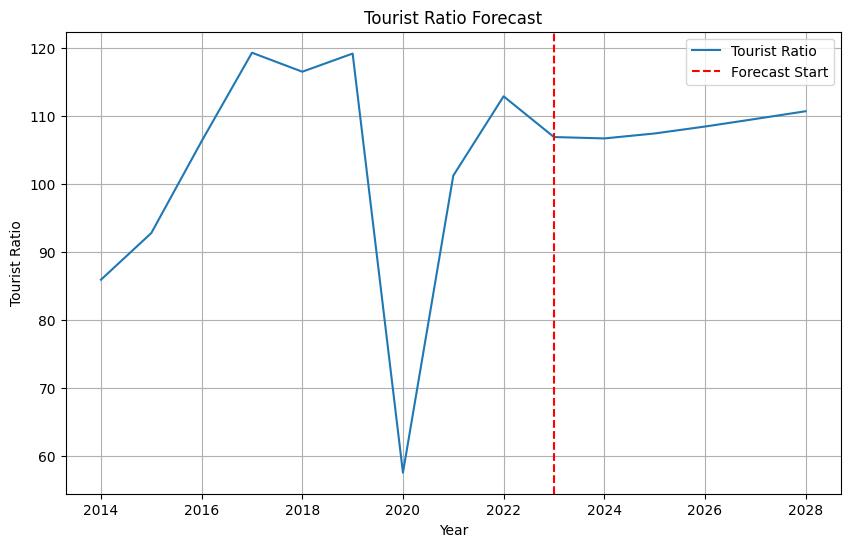
\includegraphics[width=1\textwidth]{Ratio_Sitka.png}
    \end{minipage}
    \hfill
    \begin{minipage}[t]{0.32\textwidth}
        \centering
        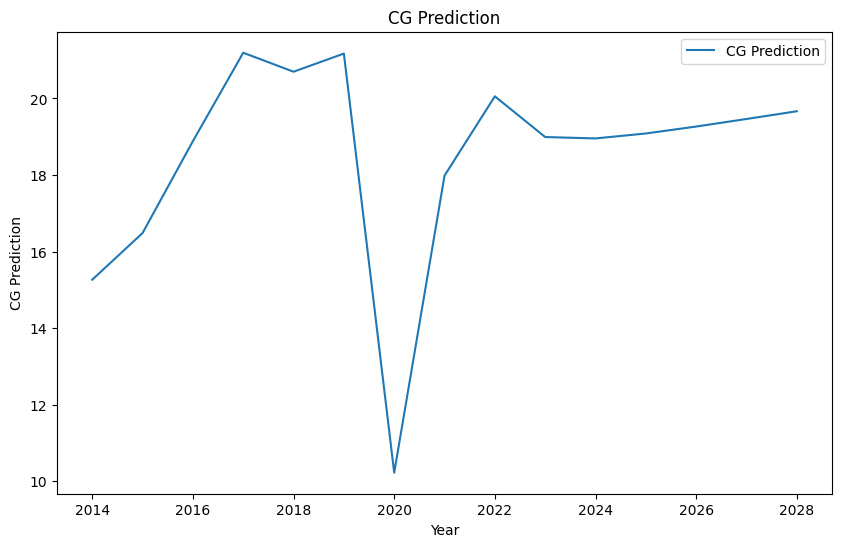
\includegraphics[width=1\textwidth]{CG_Sitka.png}
    \end{minipage}
    \hfill
    \begin{minipage}[t]{0.32\textwidth}
        \centering
        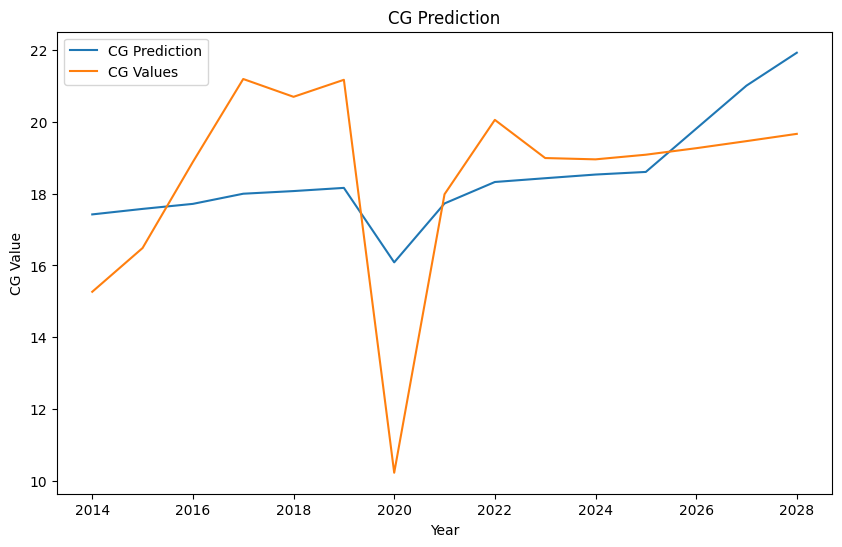
\includegraphics[width=1\textwidth]{CG_Pred_Sitka.png}
    \end{minipage}
\end{figure}

\begin{figure}[H]
    \centering
    \begin{minipage}[t]{0.32\textwidth}
        \centering
        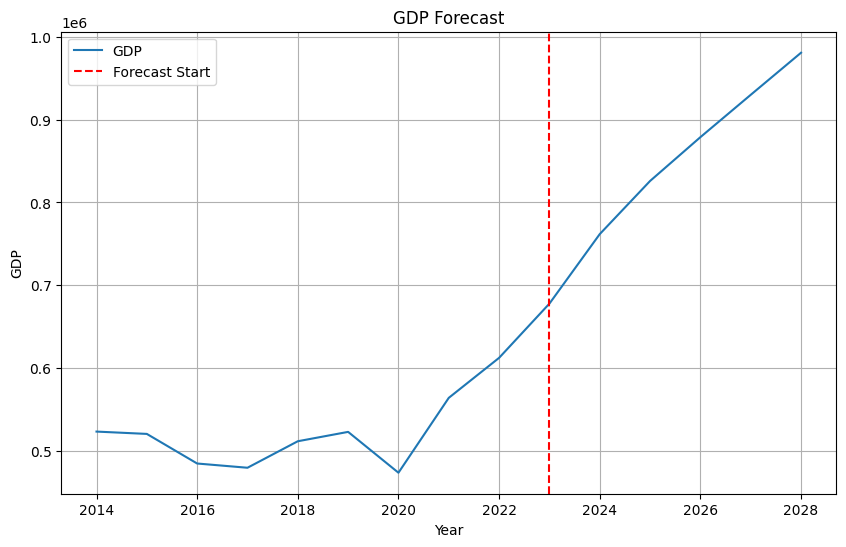
\includegraphics[width=1\textwidth]{GDP_Sitka.png}
    \end{minipage}
    \hfill
    \begin{minipage}[t]{0.32\textwidth}
        \centering
        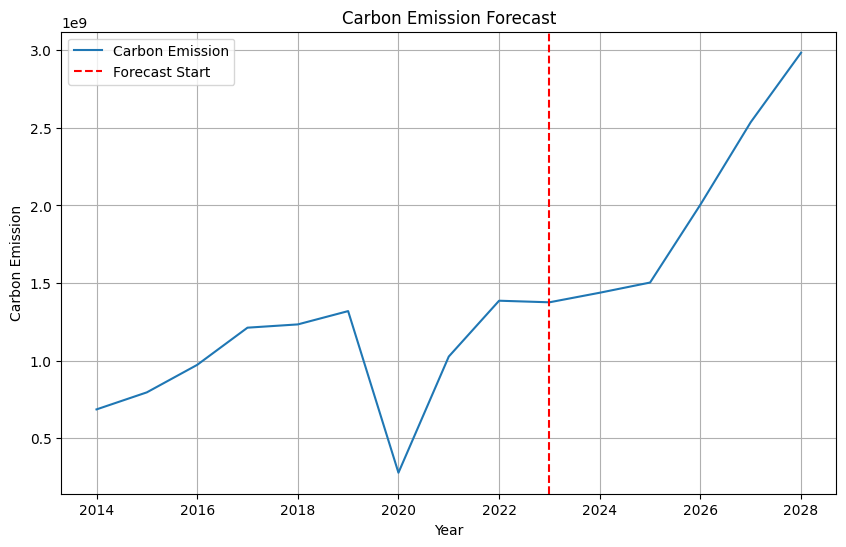
\includegraphics[width=1\textwidth]{C_Emission_Sitka.png}
    \end{minipage}
    \hfill
    \begin{minipage}[t]{0.32\textwidth}
        \centering
        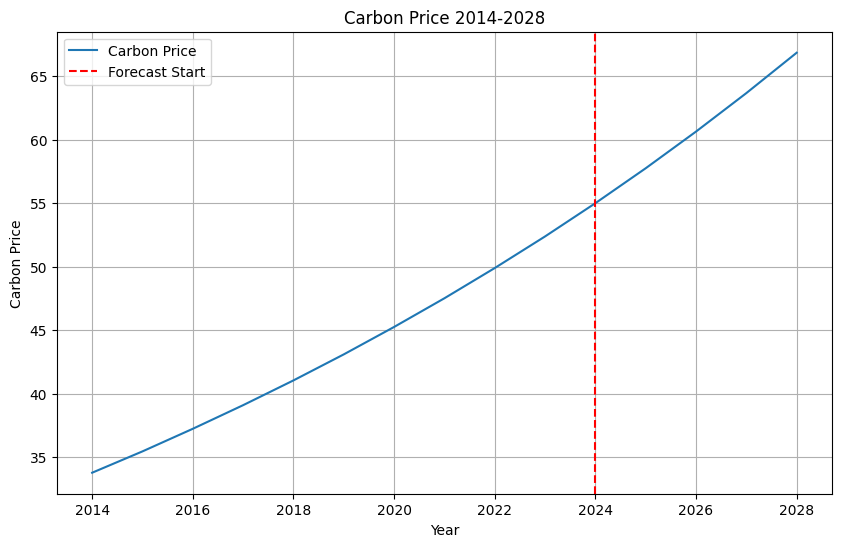
\includegraphics[width=1\textwidth]{C_Price_Sitka.png}
    \end{minipage}
\end{figure}



% \begin{figure}[H]
%     \centering
%     \begin{minipage}[t]{0.5\textwidth}
%         \centering
%         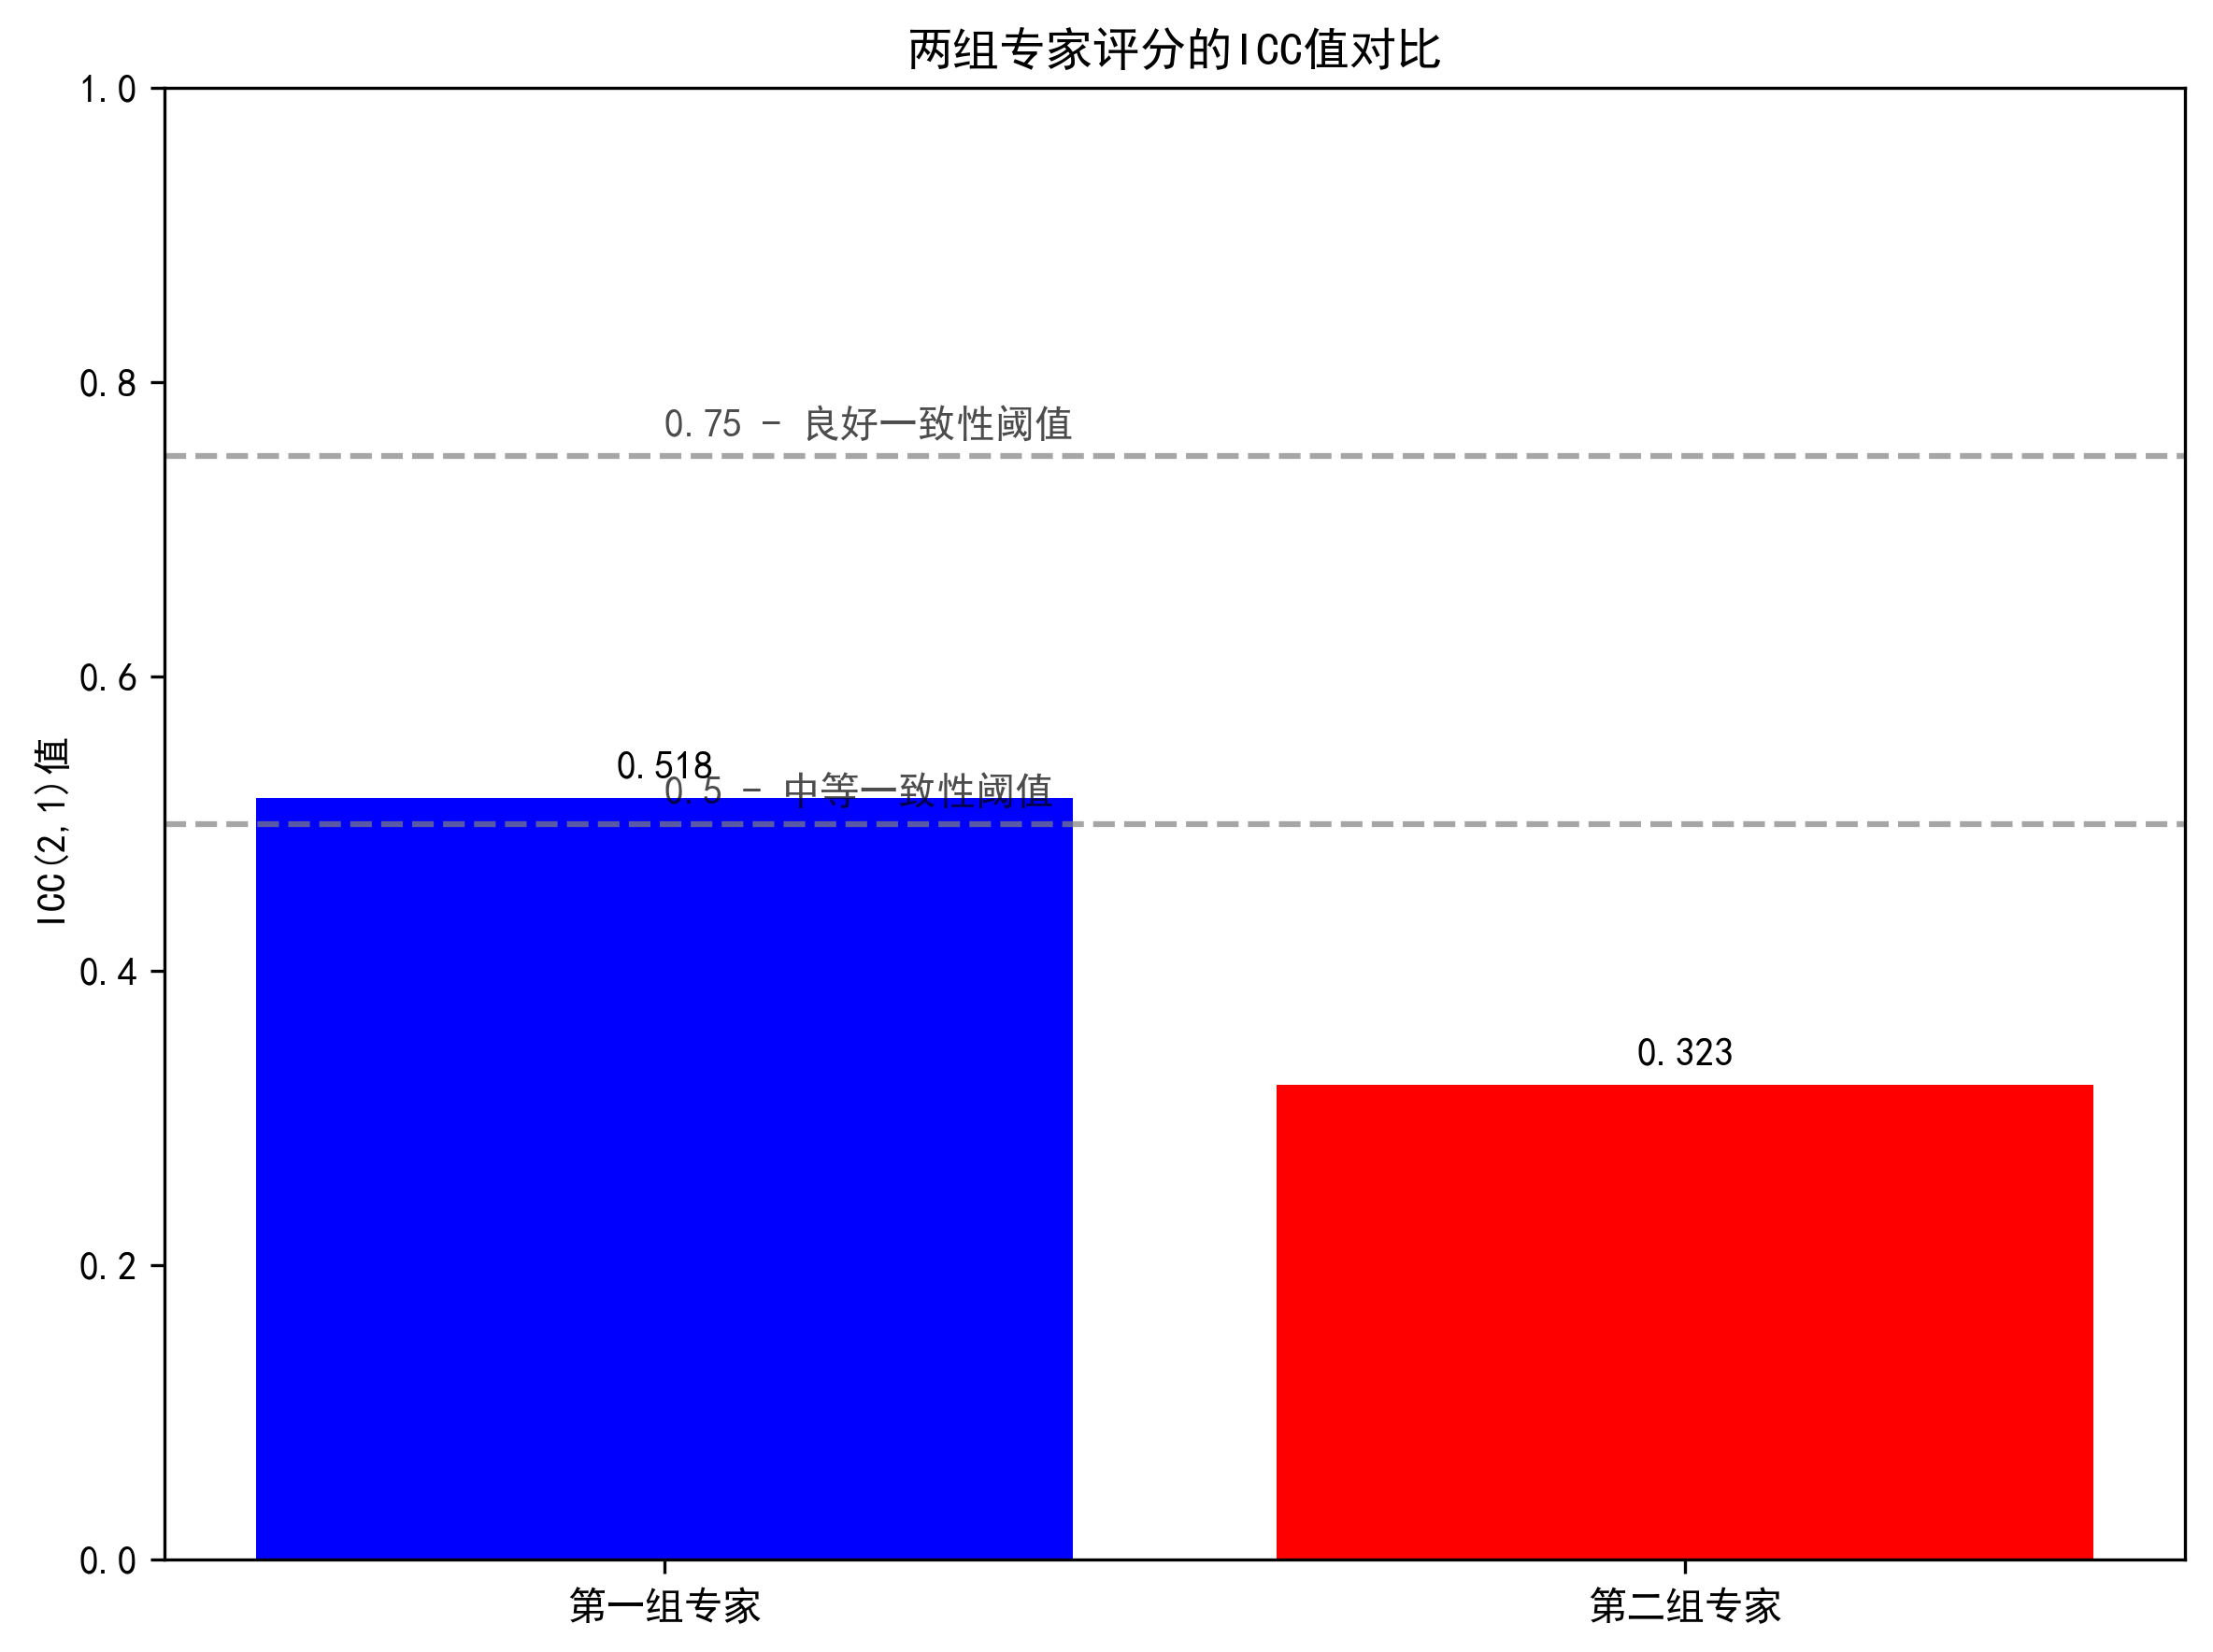
\includegraphics[width=1\textwidth]{icc_analysis.png}
%     \end{minipage}
%     \hfill
%     \begin{minipage}[t]{1\textwidth}
%         \centering
%         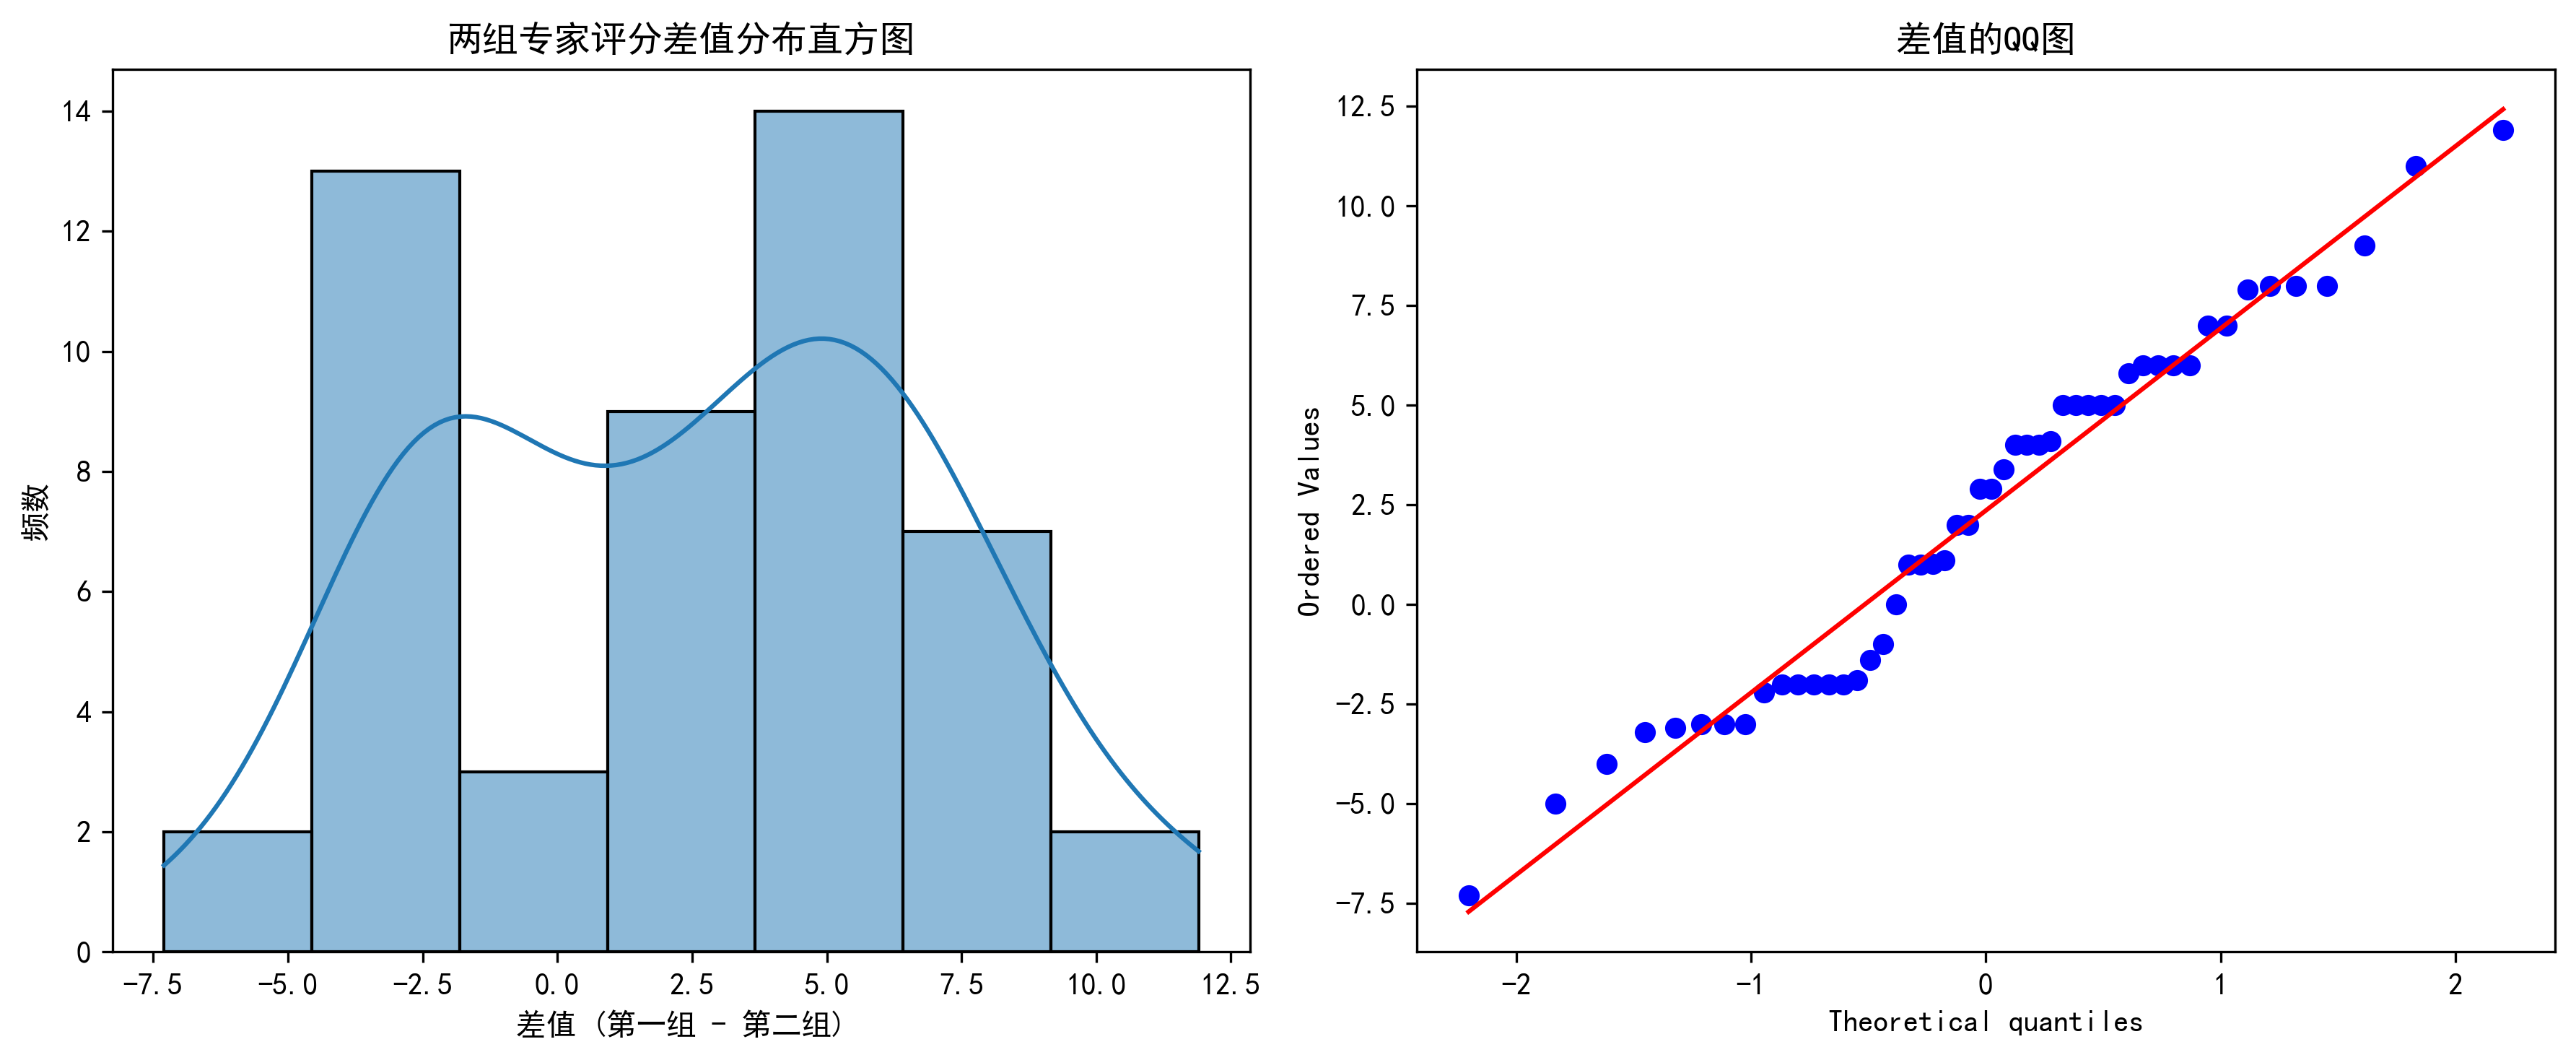
\includegraphics[width=1\textwidth]{normality_test.png}
%     \end{minipage}
% \end{figure}

\subsection{Analyses}

Summing up all the categories and the parameters yields the final equation.

\begin{equation}
    \begin{aligned}
    &\left\{\begin{array}{l}
    \mathcal{F}=(\alpha \cdot \text { Economy }-\beta \cdot \text { Environment }) / \text { Society } \\[10pt]
    \text { Economy }=165 N \cdot f(\eta) \cdot (\eta+1)+NQ\cdot e^{-0.2 Q} \\[10pt]
    \text { Environment }=2.897 \cdot N^2+ 7.67\times 10^5 N- 3.293\times 10^{10} \\[10pt]
    \text { Society }=5.011\times 10^{-9} N + 4.2 \\[10pt]
    f(\eta)=-5.5 \eta^3+9.1903 \eta^2-5.1903 \eta+1.5, \quad 0 \leq \eta \leq 1
    \end{array}\right.
    \end{aligned}
\end{equation}

When $\alpha$ is set to 1 and $\beta$ is set to 30, 
the optimal value of $N,Q,\eta$ is calculated as follows:

\begin{equation}
    \begin{aligned}
    &\left\{\begin{array}{l}
    N_{Max} = 93.353 \\[10pt]
    N_{LastYear} = 95.937 \\[10pt]
    N=52.04 \\[10pt]
    Q=4.89 \\[10pt]
    \eta=0.286
    \end{array}\right.
    \end{aligned}
\end{equation}

The strategy is the same as we have proposed in Juneau, 
that is to increase the tax rate and the fine rate, and to 
decrease the number of tourists. Thus our model can be successfully
adapted to Sitka, Alaska, proving its adaptability and migration capability.

\subsection{Sensitivity Analysis}

To evaluate the robustness of the migrated model, we conduct a sensitivity analysis.

The results are shown below:

\begin{figure}[H]
    \centering
    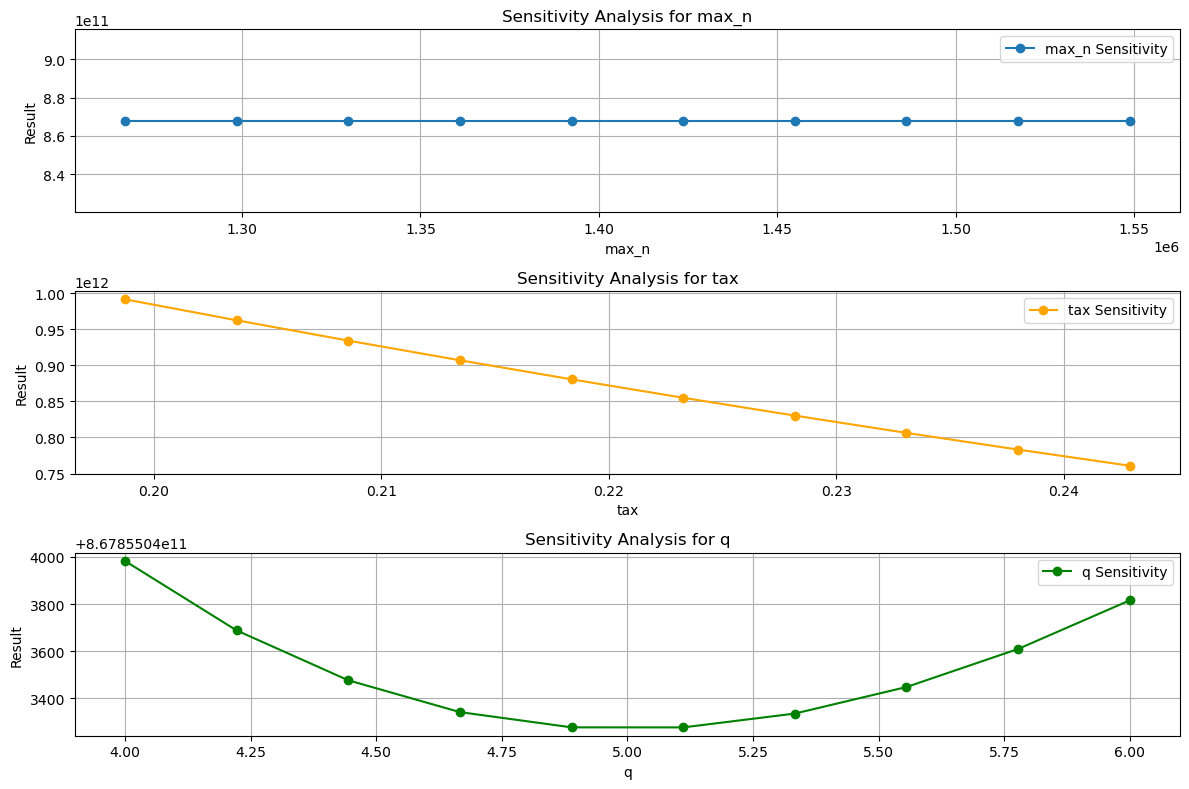
\includegraphics[width=1\textwidth]{Sensitivity_Analysis_Sitka.jpg} % 插入图片
    \vspace{-0.5cm}
    \caption{Sensitivity Analysis}
\end{figure}

It can be shown that when $N_{Max}$ is the independent variable, the outcome is immune to the change of $N_{Max}$,
while in other circumstances are sensitive to the changing of the independent variables.
The result is similar to what we conducted in Juneau.

\clearpage



\section{Task 3: Memo}
\begin{center}
    \Large\textbf{Recommendations for Sustainable Tourism in Juneau, Alaska}
\end{center}

{

Dear Tourist Council,

It is our great honour to present to you our recommendations for 
sustainable tourism in Juneau, Alaska. We have conducted a thorough 
analysis of the current situation in Juneau and have identified several key 
areas that need to be addressed in order to ensure the long-term sustainability 
of the tourism industry in the region. 
Our recommendations are based on the principles of sustainable tourism, 
which aim to balance the economic, social, and environmental impacts of tourism 
in order to ensure that it can continue to benefit both the local community and 
the environment for generations to come. Our approaches, findings and suggestions are as follows.

Firstly we summarized a general equation aiming to balance the economic, social, 
and environmental impacts of tourism. Then we looked into these aspects
and devised a model accordingly for each. \textit{SARIMAX, Linear-Regression} models 
were used to ensure the accuracy and reliability of our findings and suggestions.

Here are some findings based on our predictions.

\begin{itemize}
    \item The emission of carbon dioxide from tourism is increasing at an alarming rate, and it is 
    highly correlated with the square number of tourists.
    \item Current tax rates may not be optimal for maximizing tourism income and environmental sustainability.
    \item The number of tourists is higher than the optimal number that can be accommodated by the local environment.
\end{itemize}

Based on these findings, we put forward the following recommendations and measures.

\begin{itemize}
    \item Impose a carbon tax of around 20\% on tourism to reduce carbon emissions and encourage sustainable practices.
    \item Increase the fine amount to 20\$ for tourists who violate environmental regulations to deter harmful behavior.
    \item Set the upper limit of tourists to 1.5 million per year to protect the local environment and culture. Reduce the number of tourists by 10\% each year to around 1.2 million by 2030.
\end{itemize}

I hope you find our recommendations useful and that they will help to guide
the development of sustainable tourism in Juneau. We believe that by working
together, we can create a more sustainable future for the tourism industry in
the region. Thank you for your attention and consideration. Feel free to contact us for any further information.

\begin{flushright}
    Sincerely,\\
    Team \# 2503720 Members
    \end{flushright}

}

\clearpage

\begin{appendices}
    \section{Bivariate Linear Regression Results}

The Bivariate Linear Regression results are as follows:

\vspace{0.5cm}

    \textbf{\textit{Model for stsfy: }}

    $\text{stsfy} = -4.693528652706527 \times 10^{-5} N - 0.0060844912311383 \times N_{local} + 407.6518514$
    
    \textbf{\textit{Model for Crowding at Mendenhall Glacier: }}
    
    $\text{Crowding\_at\_Mendenhall\_Glacier} = 1.1573084349139379 \times 10^{-5} N - 0.0017873857238289111 \times N_{local} + 100.15433801$
    
    \textbf{\textit{Model for Crowding on sidewalks downtown: }}
    
    $\text{Crowding\_on\_sidewalks\_downtown} = 6.429491305077434 \times 10^{-6} N + 0.0023403412645394937 \times N_{local} - 25.69203444$
    
    \textbf{\textit{Model for Vehicle congestion downtown: }}
    
    $\text{Vehicle\_congestion\_downtown} = 2.3146168698278767 \times 10^{-5} N + 0.01642522855234218 \times N_{local} - 496.69132398$
    
    \textbf{\textit{Model for Flightseeing noise: }}
    
    $\text{Flightseeing\_noise} = -9.001287827108412 \times 10^{-6} N - 0.015276477770355294 \times N_{local} + 540.76884821$
    
    \textbf{\textit{Model for Air emissions from cruise ships: }}
    
    $\text{Air\_emissions\_from\_cruise\_ships} = -1.543077913218585 \times 10^{-5} N - 0.017616819034894794 \times N_{local} + 618.46088265$
    
    \textbf{\textit{Model for Vehicle congestion outside of downtown: }}
    
    $\text{Vehicle\_congestion\_outside\_of\_downtown} = 1.9288473915232255 \times 10^{-6} N - 0.02029789762063815 \times N_{local} + 683.19238967$
    
    \textbf{\textit{Model for Whale watching boat traffic and wakes: }}
    
    $\text{Whale\_watching\_boat\_traffic\_and\_wakes} = 1.4144880871170358 \times 10^{-5} N + 0.0011487507819868843 \times N_{local} - 12.92247577$
    
    \textbf{\textit{Model for Crowding on trails: }}
    
    $\text{Crowding\_on\_trails} = 1.2858982610154833 \times 10^{-6} N - 0.013531931747092107 \times N_{local} + 465.46159311$
    
    \textbf{\textit{Model for Street Services: }}
    
    $\text{Street\_Services} = 0.7716946724830306 \times N - 1098.7869298693258 \times N_{local} + 39720019.96870749$
    
    \textbf{\textit{Model for Wastewater: }}
    
    $\text{Wastewater} = 2.0506436350699593 \times N - 2977.4037361145515 \times N_{local} + 1.06567591 \times 10^8$
    
    \textbf{\textit{Model for Public Transit: }}
    
    $\text{Public\_Transit} = -0.11276464701428993 \times N - 1619.7640126090985 \times N_{local} + 58718764.15347296$
    
    \textbf{\textit{Model for Parks and Recreation: }}
    
    $\text{Parks\_and\_Recreation} = 2.7473696565739054 \times N - 2597.301898470375 \times N_{local} + 92393330.57040936$
    
    \textbf{\textit{Model for Docks: }}
    
    $\text{Docks} = 2.0782557994938906 \times N + 424.7535749514112 \times N_{local} - 14090559.71680191$
    
    \textbf{\textit{Model for Ports: }}
    
    $\text{Ports} = 0.708958939693741 \times N - 944.9238521963889 \times N_{local} + 33938861.95916443$
    
    \textbf{\textit{Model for JNU Composite: }}
    
    $\text{JNU\_Composite} = 9.644236957615973 \times 10^{-7} N + 0.003851051189680889 \times N_{local} + 4.69619483$
    
    \textbf{\textit{Model for Grocery Items: }}
    
    $\text{Grocery\_Items} = -2.1860270437263293 \times 10^{-5} N + 0.026042839700565677 \times N_{local} - 663.74708291$
    
    \textbf{\textit{Model for JNU Housing: }}
    
    $\text{JNU\_Housing} = -2.0702962002349386 \times 10^{-5} N + 0.0018641011281828252 \times N_{local} + 107.36835089$
    
    \textbf{\textit{Model for Utilities: }}
    
    $\text{Utilities} = 1.3951996132018008 \times 10^{-5} N + 0.008178540544050684 \times N_{local} - 142.54171473$
    
    \textbf{\textit{Model for Transportation: }}
    
    $\text{Transportation} = 1.6909562132353666 \times 10^{-5} N - 0.01094490247426114 \times N_{local} + 442.51994943$
    
    \textbf{\textit{Model for Healthcare: }}
    
    $\text{Healthcare} = -3.2147456525386777 \times 10^{-6} N + 0.006829829367730268 \times N_{local} - 59.05398278$
    
    \textbf{\textit{Model for Misc. Goods and Services: }}
    
    $\text{Misc.\_Goods\_and\_Services} = 1.9931423045740026 \times 10^{-5} N - 0.018744942079927586 \times N_{local} + 681.15469324$
    

  \end{appendices}

\clearpage

\addcontentsline{toc}{section}{References}

\begin{thebibliography}{99}
  \bibitem{mcdowell2016} McDowell Group. (2016). \textit{ Juneau Visitor Profile and Economic Impact Study}. 
  \bibitem{southeast2023} Southeast Conference. (2023).  \textit{Juneau Tourism Survey 2023}. 
  \bibitem{juneau2016} City and Borough of Juneau. (2016).  \textit{Juneau’s Visitor Industry: Positive Economic Benefits for Our Community}. 
  \bibitem{jedc2024} Juneau Economic Development Council (JEDC). (2024).  \textit{Juneau SEAK Economic Indicators and Outlook Report}. 
  \bibitem{juneau2021} City and Borough of Juneau. (2021).  \textit{Juneau Tourism Survey 2021}. 
  \bibitem{juneau2022} City and Borough of Juneau. (2022).  \textit{Juneau Tourism Survey 2022}. 
  \bibitem{juneau2023} City and Borough of Juneau. (2023).  \textit{Juneau Tourism Survey 2023}. 
  \bibitem{circulator2024} City and Borough of Juneau. (2024).  \textit{Juneau Visitor Circulator Study: Final Report}. 
  \bibitem{budget2016} City and Borough of Juneau Assembly. (2016).  \textit{Biennial Budget Fiscal Year 2016: Year 2 of the FY15/FY16 Biennial Budget}. 
  \bibitem{budget2018} City and Borough of Juneau. (2018).  \textit{Biennial Budget Adopted Fiscal Year 2018: Year 2 of the FY17/18 Biennial Budget}. 
  \bibitem{budget2020} City and Borough of Juneau. (2020).  \textit{Biennial Budget Adopted Fiscal Year 2020: Year 2 of the FY19/20 Biennial Budget}. 
  \bibitem{budget2022} City and Borough of Juneau. (2022).  \textit{Biennial Budget Adopted Fiscal Year 2022: Year 2 of the FY21/22 Biennial Budget}. 
  \bibitem{budget2024} City and Borough of Juneau. (2024).  \textit{Biennial Budget Adopted Fiscal Year 2024: Year 2 of the FY23/24 Biennial Budget}. 
  \bibitem{alaskaInventory}Alaska Department of Environmental Conservation Division of Air Quality. (2023). \textit{Alaska Greenhouse Gas Emissions Inventory}.
  \bibitem{} Alaska Municipal League (2024). \textit{State of Alaska Priority Sustainable Energy Action Plan}
  \bibitem{} UK NIR (2008). \textit{Detailed discussion of methodology and data for estimating $\mathrm{CO}_2$ emissions from fossil fuel combustion}
  \bibitem{} Final Alaska Greenhouse Gas Inventory and Reference
  Case Projections (2009). \textit{Greenhouse Gas Emissions Inventory and Reference Case Projections}
\end{thebibliography}


\clearpage

\section*{\centering Report on Use of AI}

\subsection*{GPT4o}

Messages below are conversations between a human and GPT-4o. The human is represented by \textit{Q} and GPT-4o is represented by \textit{A}.

\vspace{0.5cm}

\textit{Q1}: Write me an introduction of Juneau, Alaska. Talk about its residents, tourists and attractions.

\textit{A1}: Juneau, Alaska, the state’s capital, is a city that blends breathtaking natural beauty with rich cultural heritage. Nestled in the southeastern part of the state, Juneau is uniquely accessible only by air or sea, giving it an island-like charm despite being part of the mainland. The city is home to approximately 30,000 residents who enjoy a lifestyle deeply connected to nature, with fishing, hiking, and outdoor exploration forming an integral part of daily life.

\vspace{0.5cm}

\textit{Q2}: Can you tell me about the tourism industry in Juneau?

\textit{A2}: Juneau is a popular destination for tourists from around the world, attracting over a million visitors annually. The city’s natural wonders, including glaciers, rainforests, and abundant wildlife, make it a magnet for outdoor enthusiasts and nature lovers. Tourists can explore the Mendenhall Glacier, go whale watching, or take a scenic flight over the stunning landscape. The city also offers a vibrant arts and culture scene, with museums, galleries, and theaters showcasing the region’s history and creativity.

\vspace{0.5cm}

\textit{Q3}: What does Thousands of Chained 2017 U.S. Dollars mean?

\textit{A3}: Thousands of Chained 2017 U.S. Dollars is a measure of economic value that adjusts for inflation and changes in purchasing power over time. By using the 2017 dollar as a base year, the measure allows for more accurate comparisons of economic data across different years, accounting for the effects of inflation on prices and wages.

\vspace{0.5cm}

\textit{Q4}: What is the Kaya Identity?

\textit{A4}: The Kaya Identity is a mathematical formula used to decompose the factors driving changes in carbon dioxide emissions. It breaks down emissions into four components: population, GDP per capita, energy intensity of the economy, and carbon intensity of energy. By analyzing these factors, policymakers can identify the key drivers of emissions growth and develop strategies to reduce carbon footprints.

\vspace{0.5cm}

\textit{Q5}: Cost of converting CO2 to non-greenhouse gases?

\textit{A5}: The cost of converting CO2 to non-greenhouse gases depends on the method used and the scale of the operation. Technologies such as carbon capture and storage (CCS) and direct air capture (DAC) can be expensive due to the energy and resources required to capture and convert CO2. However, as these technologies become more advanced and widespread, the cost of converting CO2 to non-greenhouse gases is expected to decrease, making it a more viable solution for reducing emissions.

\subsection*{GPT4o-mini}

Messages below are conversations between a human and GPT4o-mini. The human is represented by \textit{Q} and 
GPT4o-mini is represented by \textit{A}.
\vspace{0.5cm}

\textit{Q6}: What does MTCO2e mean?

\textit{A6}: MTCO2e stands for metric tons of carbon dioxide equivalent, a unit of measurement used to quantify the global warming potential of greenhouse gases. By expressing emissions in terms of CO2 equivalents, different gases can be compared based on their impact on the climate, allowing for a more comprehensive assessment of a country or region’s carbon footprint.

\vspace{0.5cm}

\textit{Q7}: How to quantify the damage humans have done to the environment?

\textit{A7}: Quantifying the damage humans have done to the environment is a complex and multifaceted task that requires a combination of scientific, economic, and social analyses. Environmental impact assessments, life cycle assessments, and ecological footprint analyses are some of the tools used to measure the effects of human activities on ecosystems, biodiversity, and natural resources. By evaluating factors such as pollution, habitat destruction, and resource depletion, researchers can estimate the extent of environmental damage and develop strategies to mitigate its impact.

\end{document}
